\documentclass{article}

\usepackage{arxiv}

\usepackage[utf8]{inputenc} % allow utf-8 input
\usepackage[T1]{fontenc}    % use 8-bit T1 fonts
\usepackage{hyperref}       % hyperlinks
\usepackage{url}            % simple URL typesetting
\usepackage{booktabs}       % professional-quality tables
\usepackage{amsmath}
\usepackage{amsfonts}       % blackboard math symbols
\usepackage{nicefrac}       % compact symbols for 1/2, etc.
\usepackage{microtype}      % microtypography
\usepackage{cleveref}       % smart cross-referencing
\usepackage{graphicx}
\usepackage[round]{natbib}
\usepackage{doi}

% my packages
\usepackage{bm}
\usepackage{cancel}
\usepackage{newtxmath}

\title{A Structured Additive Multi-Species Count Model \\ for Assessing the Relation Between Site Conditions \\ and Species Diversity}

% Here you can change the date presented in the paper title
%\date{September 9, 1985}
% Or remove it
\date{}

\author{\href{https://orcid.org/0000-0003-2416-8732}{
\includegraphics[scale=0.06]{orcid.pdf}\hspace{1mm}Hannes Riebl}\thanks{The work of Hannes Riebl on this article was funded by the German Research Foundation (DFG) through the Research Training Group 2300 ``Enrichment of European Beech Forests with Conifers'' (316045089/GRK2300) and the grant ``LIESEL -- A Software Framework for Bayesian Semi-Parametric Distributional Regression'' (KN 922/11-1).} \\
  Chair of Statistics \\
  University of Göttingen \\
  Humboldtallee 3, 37073 Göttingen, Germany \\
  \texttt{hriebl@uni-goettingen.de} \\
  \And
  \href{https://orcid.org/0000-0002-7019-1899}{
\includegraphics[scale=0.06]{orcid.pdf}\hspace{1mm}Jonas Glatthorn} \\
  Bestandesdynamik und Waldbau \\
  Eidgenössische Forschungsanstalt WSL \\
  Zürcherstrasse 111, 8903 Birmensdorf, Switzerland \\
  \texttt{jonas.glatthorn@wsl.ch} \\
  \And
  \href{https://orcid.org/0000-0003-3390-0972}{
\includegraphics[scale=0.06]{orcid.pdf}\hspace{1mm}Thomas Kneib} \\
  Chair of Statistics \\
  University of Göttingen \\
  Humboldtallee 3, 37073 Göttingen, Germany \\
  \texttt{tkneib@uni-goettingen.de} \\
}

% Uncomment to override the `A preprint' in the header
%\renewcommand{\headeright}{Technical Report}
%\renewcommand{\undertitle}{Technical Report}
\renewcommand{\shorttitle}{A Structured Additive Multi-Species Count Model}

%%% Add PDF metadata to help others organize their library
%%% Once the PDF is generated, you can check the metadata with
%%% $ pdfinfo template.pdf
\hypersetup{
  pdftitle={A Structured Additive Multi-Species Count Model for Assessing the Relation Between Site Conditions and Species Diversity},
  pdfauthor={Hannes Riebl, Jonas Glatthorn, Thomas Kneib},
}

% matrices

\newcommand{\Dmat}{\mathbf{D}}
\newcommand{\Imat}{\mathbf{I}}
\newcommand{\Kmat}{\mathbf{K}}
\newcommand{\Smat}{\mathbf{S}}
\newcommand{\Tmat}{\mathbf{T}}
\newcommand{\Ymat}{\mathbf{Y}}
\newcommand{\Zmat}{\mathbf{Z}}

\newcommand{\Zeromat}{\mathbf{0}}

% vectors

\newcommand{\pvec}{\bm{p}}
\newcommand{\xvec}{\bm{x}}
\newcommand{\yvec}{\bm{y}}
\newcommand{\zvec}{\bm{z}}

\newcommand{\betavec}{\bm{\beta}}

% misc

\newcommand{\IR}{\mathbb{R}}
\newcommand{\rk}{\text{rk}}

\begin{document}
\maketitle

\begin{abstract}
We propose the multi-species count model (MSCM), a semi-parametric regression model with a novel response structure, to assess the relationship between site conditions and species diversity. The model can be applied to a broad range of problems, including the analysis of different species diversity indices and taxa. It belongs to the class of Bayesian hierarchical models, allowing us to incorporate structured additive predictors with linear, non-linear, random and spatial effects for the site conditions. The connections with several related model classes such as zero-inflated Poisson regression and multi-species occupancy models are discussed in the article, as well as a number of interesting model extensions and generalizations. We describe a robust and efficient MCMC algorithm to perform fully Bayesian inference, which we implement in Python using the probabilistic programming framework Liesel. The performance of the algorithm is illustrated in a simulation study, where we also pinpoint problematic parameter constellations in which the estimates are not well-identified. Finally, we apply the MSCM to data from the Research Training Group (RTG)~2300, a large-scale ecological research project conducted in Lower Saxony, northwest Germany, where we investigate the impact of admixing Norway spruce and Douglas fir in European beech forests, accounting for the spatial correlation of the field sites of the RTG.
\end{abstract}


% keywords can be removed
\keywords{Generalized additive model for location, scale, and shape \and Multi-species occupancy model \and Markov chain Monte Carlo simulation \and Zero-inflated data \and Spatial regression \and Structured additive predictor}


\clearpage
\section{Introduction}
\label{sec:introduction}

Loss of biodiversity due to human overuse of natural resources is one of the most pressing environmental issues of our time, as emphasized by the \citeauthor{ipbesGlobal2019} (IPBES) in its global assessment report from \citeyear{ipbesGlobal2019}. It directly impacts the integrity of ecosystems, and hence human well-being. As such, there is an urgent need for robust and effective statistical models to assess biodiversity and its drivers on local, regional and global scales. To address these questions, researchers typically collect data on the abundance of a variety of species at different field sites, together with environmental variables such as temperature, precipitation and land-use type. Analyzing such data can be a challenging task, however, as non-linear relationships and complex interactions need to be taken into account.

In large-scale ecological research projects, the assessment of biodiversity across different taxa at multiple field sites is often of primary interest. One approach to perform this analysis is to estimate the species diversity for each taxon and field site separately, based on the observed abundances, and then relate these diversity estimates to site-specific covariates using a regression model \citep{glatthornSpecies2023}. This two-step procedure has the drawback, however, that it is difficult to take the uncertainty of the diversity estimates into account in the regression model. Alternatively, a more comprehensive modeling approach is to use multi-species occupancy models \citep[MSOMs,][]{mackenzieInvestigating2004, dorazioEstimating2005}, which are a class of models that estimate the occurrence, abundance and detection probabilities of various species simultaneously, possibly allowing for interactions between them. As MSOMs involve the estimation of detection probabilities, they require repeated surveys at each field site. In meta-studies, this level of detailed data is often not available for all relevant taxa.

To address these difficulties and to provide a common model for different taxa that are monitored in a research project, we propose the novel multi-species count model (MSCM) that can be used to estimate various species diversity indices. The MSCM is formulated as a Bayesian hierarchical model, allowing us to integrate structured additive predictors with linear, non-linear, random and spatial effects of the environmental conditions at the field sites. The MSCM has a few advantages over MSOMs and other existing model classes: First, it offers a good compromise between the simplicity of a two-step analysis and the high data requirements of MSOMs, making it a suitable tool for meta-studies. Second, the formulation of the model as a directed acyclic graph (DAG) makes it straightforward to include derived quantities, i.e.~quantities that are computed from other variables in the model graph such as species diversity indices. Finally, considering the model in a Bayesian context straightforwardly allows us to compare different model specifications and assess the reliability of predictions.

We perform fully Bayesian inference using a Markov chain Monte Carlo (MCMC) algorithm, allowing us to estimate the parameters of the multi-species count model and to make predictions in a flexible and computationally efficient way. The model and inference scheme are implemented using Liesel, a probabilistic programming framework, and the corresponding MCMC library Goose \citep{rieblLiesel2022}. The software is based on the high-performance machine learning library JAX \citep{bradburyJAX2023} for Python. The robustness of the inference scheme is evaluated in an extensive simulation study. Some data-generating processes (DGPs) under which the model parameters are difficult to identify are also discussed.

Finally, we apply the MSCM to assess the species diversity of different taxa in mixed forest stands in Lower Saxony, demonstrating the flexibility of our model with a complex structured additive predictor combining parametric and non-parametric covariate effects. This way, we find that the more favorable environmental conditions at the field sites in southern Lower Saxony are reflected in a higher community diversity across all taxa. Furthermore, the diversity of the vegetation and small mammals tends to increase with the proportion of coniferous tree species at a given site.

The remainder of this article is organized as follows: Section~\ref{sec:mscm} defines the multi-species count model, including a description of structured additive predictors and the species diversity indices that can be computed from the model. Section~\ref{sec:related} explores the connections between the MSCM and other established model classes such as zero-inflated Poisson regression and multi-species occupancy models. Section~\ref{sec:inference} provides details on our fully Bayesian inference scheme, followed by a presentation of our simulation study with three scenarios in Section~\ref{sec:simulation}. In Section~\ref{sec:application}, we apply the MSCM to assess the species diversity of different taxa in mixed forest stands in Lower Saxony, before providing concluding remarks in Section~\ref{sec:conclusion}.

\section{The structured additive multi-species count model}
\label{sec:mscm}

The multi-species count model can be used with a response matrix $\Ymat$, where the entry in the $i$-th row and the $j$-th column describes how often species $j = 1, \dots, M$ was observed on experimental plot $i = 1, \dots, N$ (or more generally, on observation unit $i$). Moreover, the covariate vectors $\xvec_i$ contain information on the plots such as their geographic location, the composition of tree species or the climate. Given this sort of data, we define the multi-species count model as the following Bayesian hierarchical model with
\begin{alignat*}{3}
                        \text{the occupancy intercept of species $j$,~~~}  &&\gamma_j &\sim \text{Normal}(0, 10), \\
            \text{the probability that species $j$ occupies plot $i$,~~~} &&\psi_{ij} &=    \text{InvLogit}(\gamma_j + \eta_i), \\
\text{the unobserved indicator whether species $j$ occupies plot $i$,~~~}    &&z_{ij} &\sim \text{Bernoulli}(\psi_{ij}), \\
                         \text{the expected abundance of species $j$,~~~}     &&\mu_j &\sim \text{HalfNormal}(0, 10), \\
                  \text{the total number of observations on plot $i$,~~~}       &&n_i &\sim \text{CountDistribution}(z_{ij}, \mu_j), \\
      \text{the relative expected abundances per species on plot $i$,~~~}   &&\pvec_i &=    \frac{1}{\sum_{j=1}^M z_{ij} \mu_j} \times (z_{i1} \mu_1,\ \dots,\ z_{iM} \mu_M), \\
            \text{the number of observations per species on plot $i$,~~~}   &&\yvec_i &\sim \text{Multinomial}(n_i, \pvec_i).
\end{alignat*}
Here, the $\eta_i$ are the structured additive predictors for the plots combining different covariate effects computed from the covariate vectors $\xvec_i$ (Section~\ref{sec:predictor}). In the standard case, $\text{CountDistribution}(z_{ij}, \mu_j) = \text{Poisson}(\sum_j\lambda_{ij})$, where $\lambda_{ij} = z_{ij}\mu_j$, but other count distributions can be used to account for specific properties of the data, e.g.~the negative binomial distribution in the case of overdispersion or the Yule distribution for heavy-tailed data. Section~\ref{sec:application} presents an application where an MSCM is estimated with three different count distributions. A comparison of the models using the widely applicable information criterion (WAIC) suggests that count distributions other than the Poisson distribution often result in a better model fit. Figure~\ref{fig:rtg-graph} shows the graph of the MSCM from the application including a structured additive predictor and two species diversity indices that are derived from the model (Section~\ref{sec:diversity}).

\begin{figure}
\centering
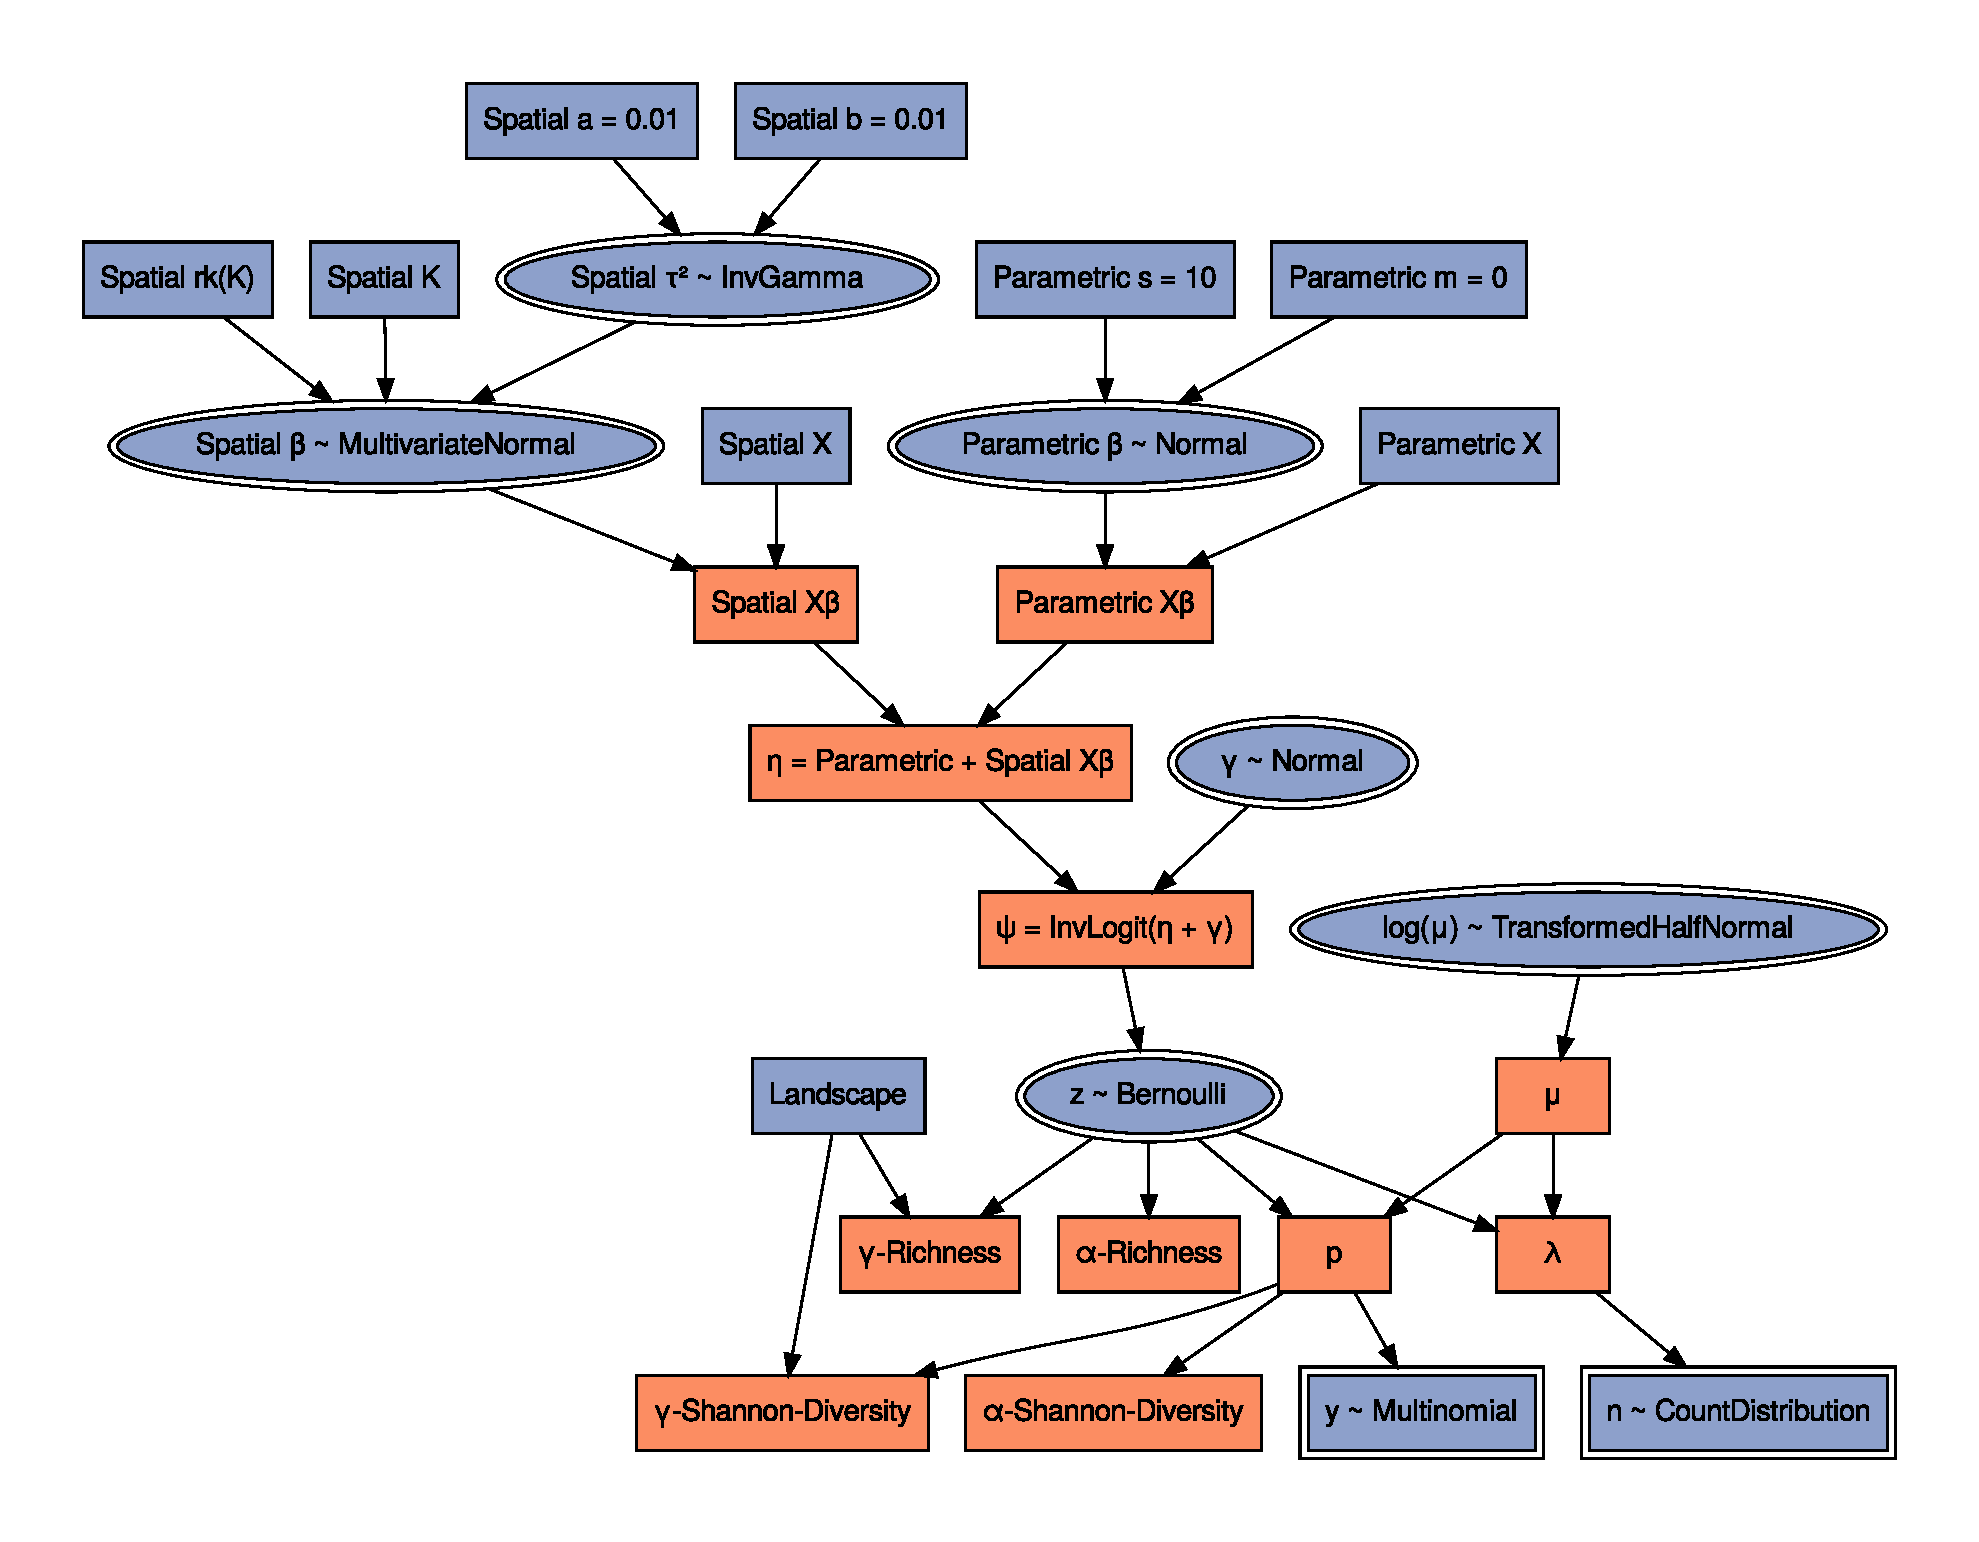
\includegraphics[width=\linewidth]{figures/rtg-graph}
\caption{The graph of the multi-species count model from the application in Section~\ref{sec:application}, implemented using the Liesel probabilistic programming framework. Blue variables are strong (constant or sampled), orange variables are weak (computed from other variables). A double contour line indicates an associated probability distribution, and a round shape indicates a model parameter. The lower part of the graph represents the response structure of the MSCM, where $n$ follows an arbitrary count distribution such as the Poisson, negative binomial or Yule distribution. The structured additive predictor $\eta$ is composed of parametric and non-parametric covariate effects. In this case, the non-parametric effect is a Gaussian process (GP) representing a spatial effect. From the response structure of the MSCM, various diversity indices such as the species richness and the Shannon index can be derived.}
\label{fig:rtg-graph}
\end{figure}

\subsection{Structured additive predictors}
\label{sec:predictor}

The structured additive predictor $\eta_i$ combines parametric covariate effects $\xvec_{i1}'\betavec_1$ and non-parametric covariate effects $f_k(\xvec_{ik}, \betavec_k)$, for $k = 1, \dots, K$, i.e.
$$\eta_i = \beta_0 + \xvec_{i1}'\betavec_1 + \sum_{k=2}^{K} f_{k}(\xvec_{ik}, \betavec_k),$$
where $\beta_0$ is the intercept and the non-parametric effects $f_k$ are centered around zero \citep[Chapter~4]{fahrmeirPenalized2004, woodGeneralized2017}. In the MSCM, the global intercept $\beta_0$ is omitted in favor of the species-specific occupancy intercepts $\gamma_j$ to ensure identifiability. The functions $f_k$ are usually modeled as linear basis expansions of the covariate vectors $\xvec_{ik}$ \citep[Chapter~5]{hastieElements2009}. Depending on the choice of the basis and the prior of the regression coefficients $\betavec_k$, the functions can represent non-linear, random and spatial effects, among others.

To avoid overfitting, certain smoothness properties of the non-parametric effects can be enforced through regularization, e.g.~using P-splines that penalize (second) differences between coefficients of neighboring B-splines \citep{eilersFlexible1996, langBayesian2004}. In a Bayesian context, regularization is accomplished using informative priors, e.g.~the multivariate normal prior
$$p(\betavec \mid \tau^2) \propto \tau^{-\rk(\Kmat)} \exp(-0.5 \tau^{-2} \betavec'\Kmat\betavec),$$
where $\tau^2$ is the variance (or smoothing) parameter, $\Kmat$ is a (potentially rank-deficient) penalty matrix, and the index $k$ is omitted for better readability. For P-splines, the penalty matrix is given by $\Kmat = \Dmat_2'\Dmat_2$, where $\Dmat_2$ is the second-order difference matrix, such that $\Dmat_2\betavec = (\beta_1 - 2\beta_2 + \beta_3,~\beta_2 - 2\beta_3 + \beta_4,~\dots)$. In this case, the penalty matrix is, in fact, rank-deficient.

Other common effect types include random effects, where the penalty matrix reduces to $\Kmat = \Imat$, (intrinsic) Gaussian Markov random field, where $\Kmat$ is determined by the underlying neighborhood structure \citep{rueGaussian2005}, and other spatial effects, where Vecchia approximations can be used to construct the penalty matrix \citep{katzfussGeneral2021}. Moreover, note that the linear effect $\xvec_{i1}'\betavec_1$ can also be embedded in this framework by setting the penalty matrix to $\Kmat = \Zeromat$, which results in a flat prior. Therefore, parametric and non-parametric effects are two sides of the same coin, and are sometimes generically referred to as predictor components or smooth terms.

For the smoothing parameter $\tau^2$, it is common to assume a weakly informative hyperprior. \citet{langBayesian2004} propose the conjugate inverse gamma prior with hyperparameters $a = b = 0.01$, or some other small value, which enables direct Gibbs updates by sampling from the full conditional. Practically, however, other priors such as the half-Cauchy distribution or the half-normal distribution may have better statistical properties \citep{gelmanPrior2006, kleinScaleDependent2016}. For a comprehensive treatment of structured additive predictors, refer to \citet{fahrmeirRegression2013}, specifically Chapter~8 and~9.

\subsection{Species diversity indices}
\label{sec:diversity}

From the multi-species count model, different biodiversity measures can be derived and estimated simultaneously with an MCMC algorithm based on one itegrated model. Among the most common biodiversity measures are the species richness and the Shannon index, both of which we assess on a plot and landscape-level in the application in Section~\ref{sec:application}.

The species richness $R_i$ of experimental plot $i$ is the total number of species that are present on that plot, i.e.
$$R_i = \sum_{j=1}^M z_{ij}.$$
As the $z_{ij}$, the indicators whether species $j$ is present at plot $i$, are unobserved and sampled with an MCMC algorithm, the species richness $R_i$ is another random variable, whose posterior distribution can be assessed from the MCMC samples. Generally speaking, species richness is a simple biodiversity measure that is easy to compute and interpret. A high species richness can be indicative of a healthy and diverse ecosystem, but as it does not take the abundances of the species into account, it can only provide an incomplete picture of biodiversity \citep{hillDiversity1973, colwellBiodiversity2009}.

The Shannon index $H'_i$, on the other hand, does take into account both the number of species and their abundances. It is computed as
$$H'_i = -\sum_{j=1}^M p_{ij} \log(p_{ij}),$$
where, by definition, some $p_{ij}$ may become zero, in which case we define $p_{ij} \log(p_{ij}) = 0$. The Shannon index $H'_i$ ranges from 0 to $\log(M)$, where $M$ is the total number of species, and provides a more complex and comprehensive biodiversity measure than the species richness $R_i$ \citep{shannonMathematical1948}. A higher Shannon index signals a greater complexity and diversity of an ecosystem.

Regardless of the specific index, species diversity can be considered on different spatial scales. The concept of $\alpha$-diversity is a measure of local biodiversity, referring to a single habitat or small area, e.g.~a 50 $\times$ 50 m$^2$ plot in the application in Section~\ref{sec:application}. In contrast, the concept of $\gamma$-diversity is defined for a larger geographic area or region, e.g.~northern or southern Lower Saxony. It is a measure of regional biodiversity and reflects the diversity of species across multiple habitats or ecosystems \citep{whittakerVegetation1960, whittakerScale2001}.

Figure~\ref{fig:rtg-graph} shows how the species richness and the Shannon index on a plot and landscape-level can be integrated into the MSCM model graph. The landscapes are defined via an $L \times N$ binary selection matrix $\Smat$, where the entry in the $l$-th~row and the $i$-th~column is one if plot $i$ belongs to landscape $l$ and zero otherwise. Based on the matrix~$\Smat$, the $\gamma$-richness can be computed as the number of non-zero entries per row of the matrix $\Tmat = \Smat\Zmat$, where $\Zmat$ is the $N \times M$~matrix containing the indicators $z_{ij}$. The $\gamma$-Shannon index can be computed in an analogous way.

\section{Related work}
\label{sec:related}

The multi-species count model is closely related to several well-known statistical and ecological model classes such as zero-inflated Poisson regression, structured additive distributional regression and multi-species occupancy models, which we discuss in more detail in this section.

\subsection{Zero-inflated Poisson regression}

Zero-inflated Poisson regression is a statistical modeling technique that can be used to analyze count data with an excess of zeros \citep{cameronRegression2013}. Mathematically, zero-inflated Poisson regression is defined as a mixture model combining a point mass at zero and a Poisson regression model. Hence, there are two possible sources of the observed zeros: the point mass and the Poisson regression model. To model the unobserved source of the observations, latent dichotomous variables are introduced, which again can be related to covariates and modeled as outcomes of another binary regression model.

Zero-inflated count data models originally were proposed by \citet{mullahySpecification1986}, together with hurdle models, another type of mixture models where zeros come from a point mass at zero as the only possible source. \citet{lambertZeroInflated1992} was the first to prominently apply zero-inflated Poisson regression to model defects in manufacturing. In addition to the covariates of the Poisson regression model, they use a logit regression model with covariates for the latent dichotomous variables describing whether the manufacturing equipment is properly aligned or not. With properly aligned equipment, defects are almost impossible, while they follow a Poisson distribution when the equipment is misaligned.

The data-generating process of the MSCM naturally falls into the category of zero-inflated count data models, as there are two possible sources of zeros: A zero occurs for sure if a plot is not occupied by a species, but it may also occur because a species is not detected despite being present at a plot. While \citet{mullahySpecification1986} notes that zero-inflated and hurdle models are equivalent if no covariates are used, this is not the case for the MSCM, where covariates are used for the occupancy probabilities.

More formally, it can be shown that the response structure of the MSCM with $\text{CountDistribution}(z_j, \mu_j) = \text{Poisson}(\sum\lambda_j)$, for $\lambda_j = z_j\mu_j$ and the species index $j = 1, \dots, M$, is, in fact, equivalent to zero-inflated Poisson regression. For one experimental plot and hence omitting the plot index $i = 1, \dots, N$, the joint probability of the observed responses and the latent occupancies of the MSCM is given by
\begin{align*}
p(\yvec, n, \zvec) &= p(\yvec \mid n, \zvec) \times p(n \mid \zvec) \times p(\zvec) \\
&= \frac{n!}{y_1! \dots y_M!} \biggl(\frac{\lambda_1}{\sum\lambda_j}\biggr)^{y_1} \dots \biggl(\frac{\lambda_M}{\sum\lambda_j}\biggr)^{y_M} \ \times \ \frac{({\sum\lambda_j})^n}{n!} e^{-\sum\lambda_j} \ \times \ \psi_1^{z_1}(1 - \psi_1)^{1 - z_1} \dots \psi_M^{z_M}(1 - \psi_M)^{1 - z_M} \\
&= \psi_1^{z_1}(1 - \psi_1)^{1 - z_1} \frac{\lambda_1^{y_1}}{y_1!} e^{-\lambda_1} \ \times \ \dots \ \times \ \psi_M^{z_M}(1 - \psi_M)^{1 - z_M} \frac{\lambda_M^{y_M}}{y_M!} e^{-\lambda_M} \ \times \ \cancel{\frac{n! ({\sum\lambda_j})^n}{n! (\sum\lambda_j)^{y_1} \dots (\sum\lambda_j)^{y_M}}}.
\end{align*}
This is the product of the probabilities of $M$ zero-inflated Poisson variables $y_j$ with the latent dichotomous variables $z_j$. As $z_j = 0 \implies y_j = \lambda_j = 0$ and $y_j = 1 \implies z_j = 0$, marginalizing out $z_j$ yields the standard probability mass function of the zero-inflated Poisson distribution, i.e.
$$
\psi_j^{z_j}(1 - \psi_j)^{1 - z_j} \frac{\lambda_j^{y_j}}{y_j!} e^{-\lambda_j} =
\begin{cases}
(1 - \psi_j) + \psi_j e^{-\lambda_j}               &\text{ if $y_j = 0$,} \\
\psi_j \frac{\lambda_j^{y_j}}{y_j!} e^{-\lambda_j} &\text{ if $y_j > 0$.}
\end{cases}
$$
Note that the equivalence depends on how the terms of the multinomial and the Poisson distribution can be rearranged. Similar operations are not possible for other count distributions such as the negative binomial or the Yule distribution, so that the equivalence does not hold in those cases.

\subsection{Structured additive distributional regression}

Zero-inflated Poisson regression and the multi-species count model belong to the so-called distributional regression model class. These models are also known as generalized additive models for location, scale and shape \citep[GAMLSS,][]{rigbyGeneralized2005}. In contrast to standard generalized linear models \citep[GLMs,][]{nelderGeneralized1972}, the response distribution of GAMLSS is not limited to the exponential family but can come from any parametric family. While the acronym GAMLSS suggests that the first three moments of the response distribution are related to covariates, this is not generally the case. For example, the two parameters of the zero-inflated Poisson distribution that are related to covariates in a regression context are the rate and zero-inflation parameter, neither of which directly represents the mean or variance of the distribution. Usually in GAMLSS, the relationship between response and explanatory variables is modeled using multiple structured additive predictors (Section~\ref{sec:predictor}). If a parameter of the response distribution is constrained, e.g.~to $(0, \infty)$ or $(0, 1)$, it needs to be transformed to $\IR$ before being linked to a structured additive predictor.

Generally, GAMLSS have the capability to accommodate a broad range of response distributions, including discrete, continuous and mixed distributions \citep{rigbyDistributions2019}. The use of various count data distributions beyond the zero-inflated Poisson distribution within the GAMLSS framework is discussed by \citet{kleinCount2015}. For non-negative continuous data, distributions like the Pareto or Weibull distribution may be a fitting choice. Regarding fractional responses, such as single or multiple percentages, \citet{kleinMultivariate2015} consider the beta and Dirichlet distributions. Finally, the GAMLSS framework can also be employed to study multivariate responses, using either conventional multivariate distributions \citep{michaelisBayesian2018} or copulas to describe complex dependence structures with arbitrary marginal distributions \citep{kleinSimultaneous2016}.

In a recent review paper, \citet{stasinopoulosGAMLSS2018} provide an overview of the scientific fields where GAMLSS have been applied since their introduction by \citeauthor{rigbyGeneralized2005} in \citeyear{rigbyGeneralized2005}. The fields include biology \citep{hawkinsIncreasing2013}, economics \citep{voudourisEconomic2015}, environmental science \citep{villariniFlood2009}, genomics \citep{khondokerComparison2007}, management science \citep{budgeEmpirical2010} and medicine \citep{rodriguesCOM2009}. A Bayesian workflow for GAMLSS is described by \citet{umlaufPrimer2018} together with an application on German weather data.

\subsection{Multi-species occupancy models}

As the name suggests, the multi-species count model is also closely linked to multi-species occupancy models, a widely-used method in ecology for estimating the probabilities of occurrence and detection of multiple species at the same time. Multi-species occupancy models (MSOMs) were first introduced by \citet{mackenzieInvestigating2004} and \citet{dorazioEstimating2005} as an extension of single-species occupancy models, and they have gained significant popularity in recent years. MSOMs are commonly used to study the composition and diversity of species communities, as the joint analysis of data on multiple species is often more effective and informative than modeling each species separately \citep{devarajanMultispecies2020}.

As MSOMs involve the estimation of detection probabilities, they require data from multiple surveys per field site \citep{devarajanMultispecies2020}. This is an essential difference between MSOMs and our model, which relies on a single count per species and field site and hence does not require repeated surveys. As the data requirements of our model are relatively low, it is a good tool for meta-studies on various taxa, even if the species are sampled according to different protocols for each taxon. On the other hand, our model is not designed to disentangle if differences in the recorded counts are due to differences in the abundances or the detection probabilities of the species. Hence, when species diversity indices are computed from our model, the implicit assumption is that the counts are proportional to the abundances, i.e.~that the detection probability is constant across all species.

Some variants of MSOMs can take biotic interactions between species into account. Correlations between occurrence probabilities of different species are often a result of shared habitat requirements and similar responses to relevant environmental factors. By including such dependencies in the model, the accuracy of the occupancy estimates can be improved, and the mechanisms driving co-occurrence patterns can be better understood. Specific MSOMs with a focus on species co-occurrence and biotic interactions have been developed by \citet{mackenzieInvestigating2004}, \citet{waddleNew2010} and \citet{rotaMultispecies2016}.

In the form presented in Section~\ref{sec:mscm}, our model cannot take biotic interactions between species into account. However, it would be straightforward to equip the model with this feature, e.g.~by introducing a multivariate normal prior for the species-specific occupancy intercepts $\gamma_j$ and the expected abundances $\lambda_j$. This way, a suitable correlation structure between the species could be enforced. The researcher could either fix or estimate the correlations, depending on the specific parameterization of the model. One drawback of estimating the correlations would be an increased number of parameters, which could potentially result in identification issues and increase the computational cost of the model. If the correlations were specified in the most naive way, the number of parameters would increase quadratically with the number of species, i.e.~sparse parameterizations would become necessary for more than four or five species. In fact, most MSOM variants with a focus on co-occurrence patterns are limited to a relatively small number of species \citep{devarajanMultispecies2020}.

Some MSOMs can also be used to estimate the size of an unobserved meta-community. For this purpose, \citet{dorazioEstimating2005} propose a parameter-expanded data augmentation technique for MCMC inference, where some all-zero columns representing potentially unobserved species are added to the response matrix $\Ymat$. The size of the meta-community is then assessed by estimating the number of extra columns \citep{keryBayesian2012}. Our model as described in this article lacks the ability to quantify the size of the meta-community, i.e.~all relevant species must be added to the response matrix $\Ymat$ by the researcher.

Due to the high degree of flexibility in terms of the model specification, presenting MSOMs concisely can be a challenging task for researchers. \citet{devarajanMultispecies2020} provide a review of 92 studies using MSOMs that were published between 2009 and 2018, spanning 27 countries and various taxa. They observe a consistent pattern of underreporting on aspects as diverse as the spatial and temporal scope of the data, the field methods and the type of detectors, as well as the covariates and the statistical tools. The insufficient reporting undermines the robustness of the inferences and the reproducibility of the studies, and could potentially have an adverse effect on conservation and management efforts.

Many studies using MSOMs also lack an explicit discussion of the model assumptions. \citet{devarajanMultispecies2020} note, for example, that monitoring is usually geared towards one focal species, and other species are only recorded as bycatch. If MSOMs are used with such data, the assumptions are unlikely to transfer seamlessly between the focal and the bycatch species. Despite the biases and errors associated with MSOMs involving bycatch data, only about a quarter of the studies reviewed by \citeauthor{devarajanMultispecies2020} mention the presence of bycatch species in the study area.

\section{Bayesian inference}
\label{sec:inference}

A variety of approaches exist for Bayesian inference in distributional regression with structured additive predictors. To assess the posterior distribution of the model parameters, \citet{kleinCount2015} propose a MCMC algorithm using a Metropolis-within-Gibbs scheme with iterative weighted least squares \citep[IWLS, ][]{gamermanSampling1997} proposals for the parametric and non-parametric regression coefficients $\beta$. The IWLS proposals are locally adaptive and make use of the expected or observed Fisher information to construct proposal densities that approximate the curvature of the posterior. For this reason, they are useful for complex posteriors, and at the same time, they do not require the user to tune any hyperparameters of the MCMC algorithm.

In combination with the IWLS proposals, the algorithm of \citet{kleinCount2015} uses conjugate inverse gamma priors for the smoothing parameters $\tau^2$ of the non-parametric covariate effects. Assuming an inverse gamma prior with the hyperparameters $a$ and $b$ for $\tau^2$, the smoothing parameter can be sampled directly from the full conditional $\tau^2 \mid \cdot \sim \text{InvGamma}(a^*, b^*)$, where $a^* = 0.5 \times \text{rk}(\Kmat) + a$, $b^* = 0.5 \times \betavec'\Kmat\betavec + b$, $\Kmat$ is the penalty matrix, and $\betavec$ are the regression coefficients of the covariate effect.

As the IWLS proposals involve second derivatives, they tend to become computationally expensive and numerically unstable if many parameters are sampled together. A popular alternative is the Hamiltonian Monte Carlo \citep[HMC, ][]{nealMCMC2011} algorithm that simulates the evolution of a Hamiltonian system, defined by a potential and a kinetic energy function, using numerical integration methods to generate posterior samples. To simulate this motion of particles, only the gradient of the log-posterior but no second derivatives are required. Based on the trajectory, new values for the model parameters are proposed, which are finally accepted or rejected in a Metropolis-Hastings step.

To explore the posterior distribution efficiently, the user needs to find a suitable value for the number of leapfrog steps of the HMC algorithm. To eliminate the requirement of tuning the number of leapfrog steps, the No-U-Turn Sampler (NUTS) was developed as a variant of HMC by \citet{hoffmanNoUTurn2014}. NUTS uses a recursive algorithm to build a binary tree of possible states and to adjust the trajectory of the particles in a dynamic way responding to the curvature of the posterior. For this reason, NUTS is typically easier to use and more efficient than HMC or other traditional MCMC methods.

Our approach to estimate the MSCM combines a Metropolis-within-Gibbs scheme with NUTS, using the same way to block the parameter vector as \citet{kleinCount2015} but exchanging the IWLS updates of the parametric and non-parametric regression coefficients $\beta$ with NUTS updates. For the smoothing parameters $\tau^2$ of the non-parametric covariate effects, we use conjugate inverse gamma priors, allowing us to sample directly from the full conditionals. Additionally, the occupancy states $z$ are sampled in a Gibbs update, and for the species-specific expected abundances $\log(\mu)$ and the occupancy intercepts $\gamma$, two separate NUTS updates are performed. More systematically, our MCMC algorithm can be described as follows:

\begin{enumerate}
\item Initialize the model parameters as $z = \bm{1}(y > 0)$, where $\bm{1}$ is the indicator function, $\mu = [\sum_{i=1}^N y_i \times \bm{1}(y_i > 0)] / [\sum_{i=1}^N \bm{1}(y_i > 0)]$, i.e. the mean of the non-zero counts for one species over the sites, $\gamma = 0$, $\beta = 0$ and $\tau^2 = 10.000$.
\item For each iteration of the algorithm:
  \begin{itemize}
  \item Sample the occupancy states $z$ from the binary full conditional in a Gibbs update.
  \item Update the species-specific expected abundances $\log(\mu)$ using NUTS.
  \item Update the species-specific occupancy intercepts $\gamma$ using NUTS.
  \item Update the site-specific parametric regression coefficients $\beta$ using NUTS.
  \item For each site-specific non-parametric covariate effect:
    \begin{itemize}
    \item Update the non-parametric regression coefficients $\beta$ using NUTS.
    \item Sample the smoothing parameter $\tau^2$ from the inverse gamma full conditional in a Gibbs update.
    \end{itemize}
  \end{itemize}
\item Repeat step 2 for a great number of iterations to obtain a representative sample from the posterior distribution of the model parameters.
\end{enumerate}

The proposed sampling scheme is designed to iterate over the parameter variables in the model graph from the bottom to the top, so that the highest level of the prior hierarchy is sampled last. The scheme is illustrated in Figure~\ref{fig:rtg-mcmc} for the MSCM used in the application in Section~\ref{sec:application}. To implement the scheme, we use Goose, the MCMC library of the probabilistic programming framework Liesel, which among other MCMC kernels, provides the NUTS kernel and an abstract Gibbs kernel \citep{rieblLiesel2022}. Using Goose, only the methods to sample from the full conditionals of the model parameters $z$ and $\tau^2$ need to be implemented manually.

To improve the performance of the sampling scheme, we run it in two phases: a warmup and a posterior phase. During the warmup, the NUTS kernels are allowed to tune their hyperparameters, i.e.~the step size and the mass matrix (also called metric). To tune the step size in an adaptive way, we use the dual averaging algorithm, which increases or decreases the step size based on the acceptance probabilities of the previous iterations, hence improving the convergence rate and reducing the dependence on user-defined hyperparameters \citep{hoffmanNoUTurn2014, nesterovPrimaldual2009}. The mass matrix, on the other hand, is supposed to capture correlations in the posterior and is tuned based on the empirical covariance of the warmup samples. A well-adjusted mass matrix can improve the mixing and convergence rate of the HMC and NUTS algorithms substantially in many situations \citep{betancourtConceptual2018}.

In our experience, the proposed sampling scheme is robust and efficient for many different parameters of the data-generating process of the MSCM. More details on the accuracy and performance of the MCMC algorithm are given in the simulation study in the following section.

\begin{figure}
\centering
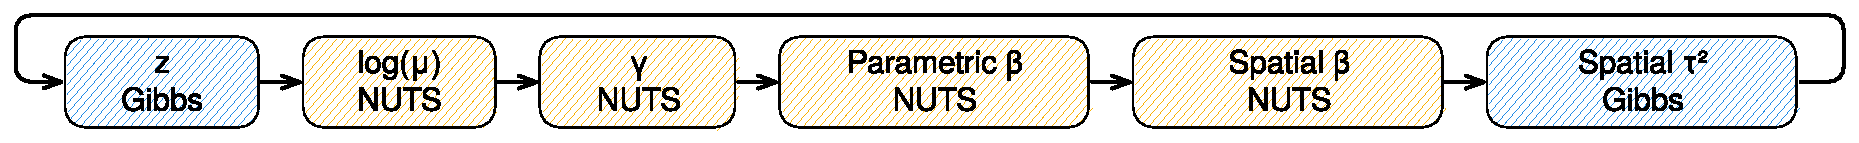
\includegraphics[width=\linewidth]{figures/rtg-mcmc}
\caption{The proposed MCMC sampling scheme for the multi-species count model, illustrated for the model graph in Figure~\ref{fig:rtg-graph}. The algorithm iterates over the parameter variables in the model graph from the bottom to the top, so that the highest level of the prior hierarchy is sampled last. Generally, the structured additive predictor $\eta$ of an MSCM can include more than one non-parametric covariate effect, i.e.~there could be additional NUTS and Gibbs kernels for the $\beta$ and $\tau^2$ parameters of all non-linear, random and spatial effects.}
\label{fig:rtg-mcmc}
\end{figure}

\section{Simulation study}
\label{sec:simulation}

We examine our sampling scheme in a simulation study with three scenarios: In the first scenario, we confirm that the MCMC algorithm is able to recover the true model parameters reliably in most practically relevant situations. The second scenario is designed to produce more extreme data, i.e.~data where the model parameters are closer to the boundaries of the parameter space. We use this data to evaluate the performance of the MCMC algorithm under more challenging conditions. Finally, we demonstrate that the sampling scheme also works with structured additive predictors and spatial effects in Scenario~III.

To conduct the simulation study, we generate data from the MSCM, adopting the priors of the model parameters to produce more or less extreme parameters and therefore data. For each scenario, we run 1000 replications, generating four independent chains with 1000 warmup and 1000 post-warmup samples per replication. No thinning is applied to the chains before they are used to compute the summary statistics of the posterior. Various metrics such as the bias, the root-mean-square error (RMSE) and the coverage probability are used to assess the performance of the sampling scheme.

We find that our method works accurately under realistic conditions with and without structured additive predictors. If the occupancy probability $\psi$ is close to zero or one and the expected abundance $\mu$ of a species is small, the estimated posterior mean of the species-specific occupancy intercept $\gamma$ tends to show some bias. However, the posterior standard deviation also increases drastically in these cases, indicating a high uncertainty about the estimate, so that the issue can easily be identified from the MCMC output.

\subsection{Scenario I: Stable MCMC estimation}

In the first scenario, we demonstrate that our sampling scheme is able to recover the true parameters of the MSCM. For this purpose, we simulate data from the MSCM as defined in Section~\ref{sec:mscm}, exchanging the weakly informative priors of the species-specific occupancy intercepts $\gamma$ and the expected abundances $\mu$ with narrower sampling distributions as follows:
\begin{align*}
\beta, \gamma &\sim \text{Normal}(\mu = 0,\ \sigma = 0.5), \\
          \mu &\sim \text{Gamma}(\alpha = 10,\ \beta = 1).
\end{align*}
We also simulate two independent site-specific covariates from a uniform distribution on the unit interval. This configuration implies that the true occupancy probabilities $\psi$ are between 17.6\% and 82.3\% and the true expected abundances $\mu$ are between 4.1 and 18.8 with 99\% probability (see Table~\ref{tab:sim-truth}). Despite the modified data-generating process, we use the weakly informative priors from Section~\ref{sec:mscm} for the estimation to encode less knowledge about the DGP in the priors and to estimate the model in the exact same way as in the application in Section~\ref{sec:application}.

\begin{table}
\centering
\caption{The quantiles of the simulated true model parameters in the different scenarios of the simulation study. Scenario~I and~III are designed to produce realistic data with and without structured additive predictors. In Scenario~II, the performance of the sampling scheme is assessed when the model parameters are close to the boundaries of the parameter space.}
\label{tab:sim-truth}
\begin{tabular}{llrrrrrr}
\toprule
                                      &           & \multicolumn{2}{c}{Scenario I} & \multicolumn{2}{c}{Scenario II} & \multicolumn{2}{c}{Scenario III} \\
                                                    \cmidrule(lr){3-4}               \cmidrule(lr){5-6}                \cmidrule(lr){7-8}
Parameter                             &           &      1\% &     99\%            &      1\% &     99\%             &      1\% &     99\% \\
\midrule
Parametric regression coefficients    & $\beta$   & $-1.175$ &  $1.178$            & $-2.241$ &  $2.399$             & $-1.152$ &  $1.174$ \\
Spatial regression coefficients       & $\beta^s$ &      --- &      ---            &      --- &      ---             & $-2.312$ &  $2.327$ \\
Species-specific occupancy intercepts & $\gamma$  & $-1.166$ &  $1.170$            & $-2.337$ &  $2.328$             & $-1.164$ &  $1.204$ \\
Species-specific expected abundances  & $\mu$     &  $4.141$ & $18.768$            &  $0.142$ & $26.029$             &  $4.185$ & $18.781$ \\
Occupancy probabilities               & $\psi$    &  $0.176$ &  $0.823$            &  $0.047$ &  $0.957$             &  $0.120$ &  $0.883$ \\
\bottomrule
\end{tabular}
\end{table}

For each of the sample sizes of 40 and 80 sites, and 26 and 52 species, our method is able to recover the true parameters without problems. The estimated posterior means computed from the MCMC chains are unbiased on average, and the bias shrinks with the sample size (see Figure~\ref{fig:sim-1-bias}). A greater sample size affects the estimation of the various model parameters in different ways: The regression coefficients $\beta$ benefit from more sites and more species, because they are shared between the sites and the species. On the other hand, the estimation of the occupancy intercepts $\gamma$ and the expected abundances $\log(\mu)$ can only be improved with more sites, not more species, because they are not shared between the species.

\begin{figure}
\centering
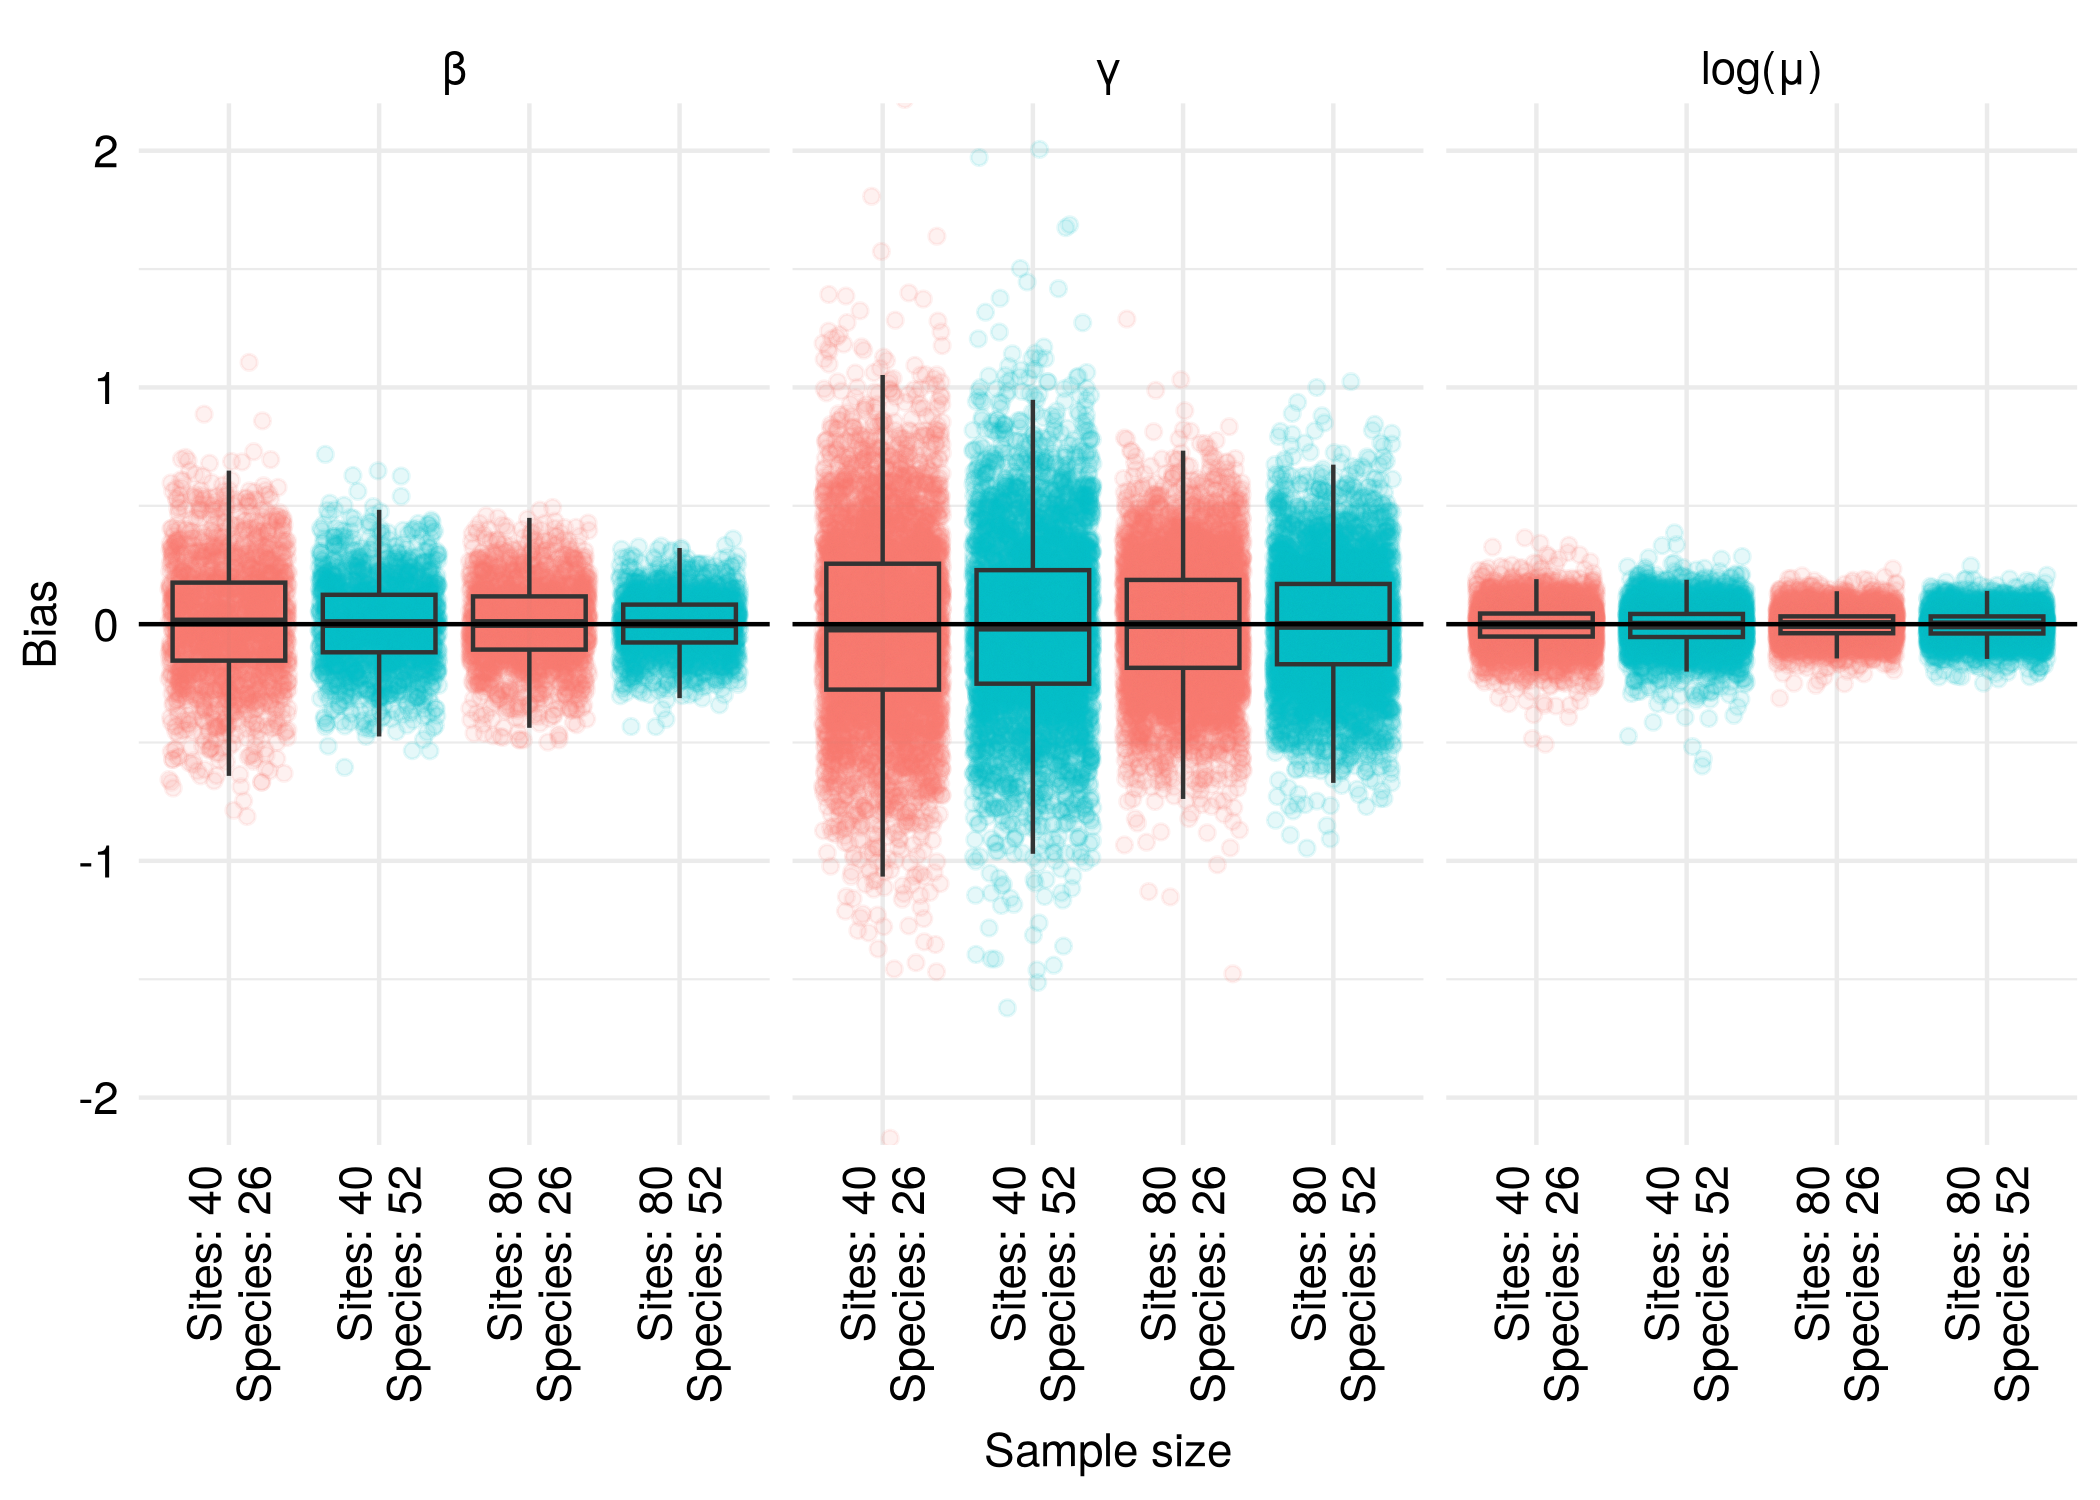
\includegraphics[width=.7\linewidth]{figures/sim-1-bias}
\caption{The bias of the estimated posterior mean of the model parameters for 1000 replications of Simulation Scenario~I. The average bias is close to zero for all model parameters and sample sizes. Most variability is observed in the bias of the species-specific occupancy intercepts $\gamma$, followed by the site-specific regression coefficients $\beta$ and the species-specific expected abundances $\log(\mu)$. The bias of the regression coefficients $\beta$ decreases with both the number of sites and species, while the estimation of the occupancy intercepts $\gamma$ and the expected abundances $\log(\mu)$ only benefits from more sites but not more species.}
\label{fig:sim-1-bias}
\end{figure}

\subsection{Scenario II: Problematic parameter constellations}

This simulation scenario includes more cases where the model parameters are close the boundaries of the parameter space, posing a more challenging estimation problem to our MCMC algorithm. To generate this kind of data, we sample the model parameters from the distributions
\begin{align*}
\beta, \gamma &\sim \text{Normal}(\mu = 0,\ \sigma = 1), \\
          \mu &\sim \text{HalfNormal}(\sigma = 10).
\end{align*}
Again, we simulate two site-specific covariates on the unit interval using a uniform distribution. In this scenario, the true occupancy probabilities $\psi$ are between 4.7\% and 95.7\% and the true expected abundances $\mu$ are between 0.1 and 26.0 with 99\% probability (Table~\ref{tab:sim-truth}). The usual weakly informative priors are used for the estimation.

From 1000 replications with 40 sites and 26 species, we find that the average bias of the estimated posterior mean is still close to zero for all model parameters, but for the species-specific occupancy intercepts $\gamma$ and the expected abundances $\log(\mu)$, it increases substantially compared to Scenario~I ($0.025$ vs.~$-0.010$ for~$\gamma$, and $0.049$ vs.~$-0.006$ for~$\log(\mu)$). In particular, there are several cases when $\gamma$ is strongly underestimated (when its true value and the true $\mu$ are small), and when it is strongly overestimated (when its true value is large but the true $\mu$ is small, see Figure~\ref{fig:sim-2-gamma}). In these cases, the posterior standard deviation also increases drastically, indicating a high uncertainty about the estimate. For this reason, the coverage rates of the 90\% credible intervals remain relatively stable with 86.5\% for $\gamma$ and 86.7\% for $\log(\mu)$.

The difficulties with these parameter constellations are to be expected considering their interpretation: A low expected abundance $\mu$ implies that few or no individuals are observed at each site, no matter if the site was occupied by the species or not. Under these circumstances, it is hard to disentangle whether an observed zero is the result of a low occupancy probability or a low expected abundance, and hence the species-specific occupancy intercept $\gamma$ is not well-identified. Finally, it is worth mentioning that despite the bias in the estimation of $\gamma$, the occupancy probabilities $\psi$ including the site-specific regression coefficients $\beta$ are still estimated quite accurately on the unit interval after the inverse logit transformation.

\begin{figure}
\centering
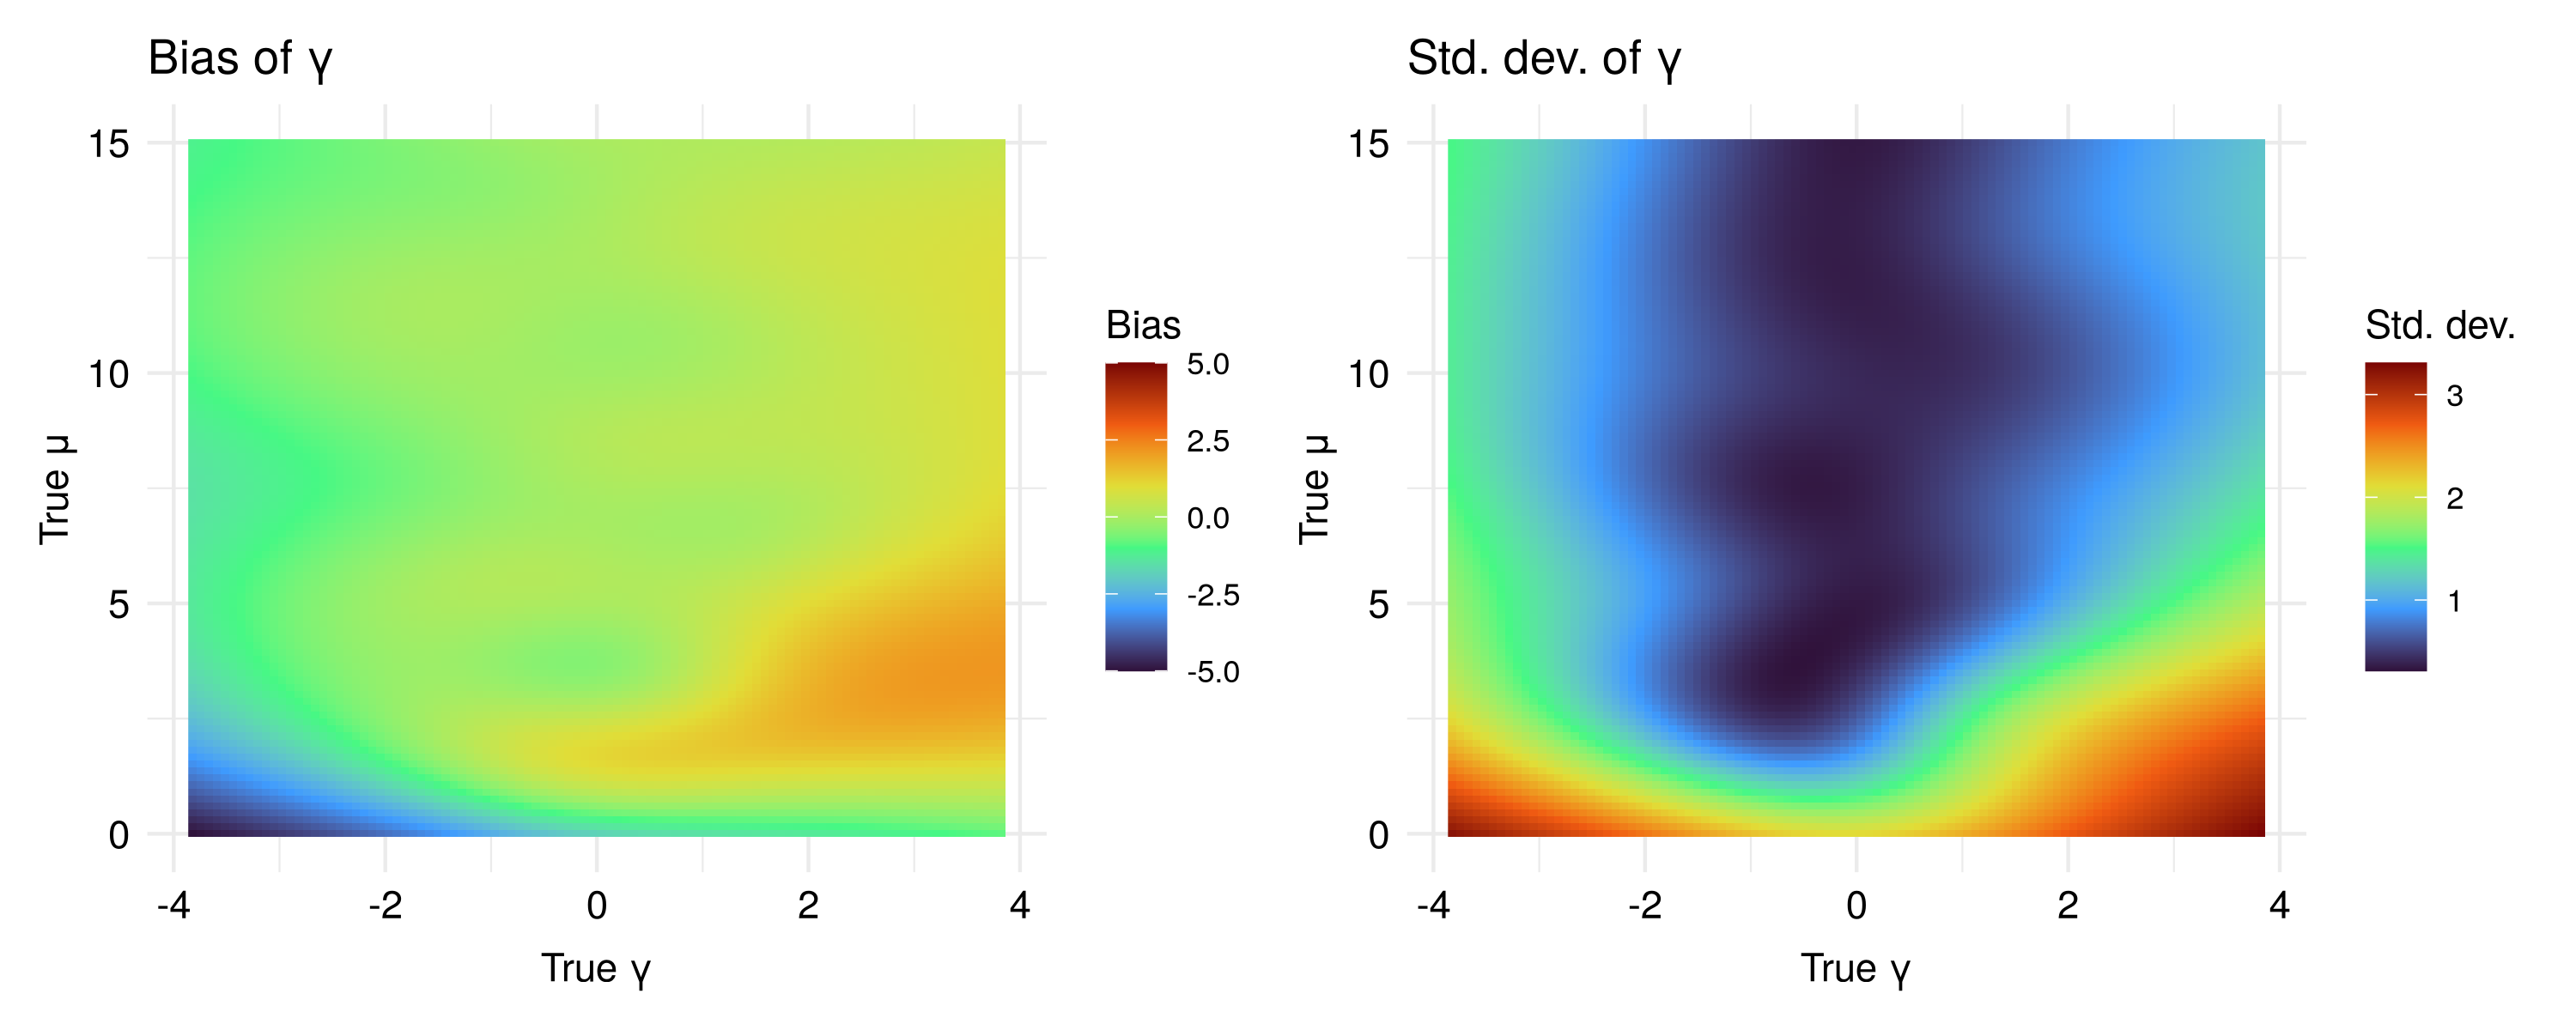
\includegraphics[width=\linewidth]{figures/sim-2-gamma}
\caption{The bias of the estimated posterior mean (left) and the estimated posterior standard deviation (right) of the species-specific occupancy intercept $\gamma$ as a function of the true occupancy intercept $\gamma$ and the true expected abundance~$\mu$ in Simulation Scenario~II. If the abundance and the occupancy are small, $\gamma$ tends to be underestimated, while it tends to be overestimated if the abundance is small but the occupancy is large. In these cases, the posterior standard deviation also increases drastically, indicating a high uncertainty about the estimate.}
\label{fig:sim-2-gamma}
\end{figure}

\subsection{Scenario III: Structured additive predictors}

In the last scenario, we verify that our sampling scheme also works with the model structure used in Section~\ref{sec:application}, i.e.~with a structured additive predictor and a spatial effect. The spatial effect is modeled as a latent Gaussian process with a Matérn correlation function and a fixed smoothness parameter $\nu = 1.5$. The simulated data comprises 40 sites and 26~species. The 40 sites are geographically clustered in the same way as in Section~\ref{sec:application}, resulting in a similar correlation matrix as in Figure~\ref{fig:rtg-correlation}. In addition to the spatial effect, this scenario also includes two continuous covariates on the unit interval with parametric linear effects. The spatial regression coefficients are sampled from an improper multivariate normal distribution with the smoothing parameter $\tau^2 = 1$, and all other model parameters are sampled from the same distributions as in Scenario~I.

Although there are substantially more parameters than in Scenario~I, our method is able to estimate the spatial effect reliably. The average bias of the estimated posterior mean of the spatial regression coefficients ($0.005$) is on a similar scale as the bias of the parametric regression coefficients ($-0.001$). The bias of the parametric regression coefficients does not increase compared to Scenario~I ($-0.001$ vs. $0.011$ in Scenario~I). Moreover, the coverage rates of the 90\%~credible intervals of the spatial regression coefficients are remarkably accurate (90.1\%). Only the smoothing parameter~$\tau^2$ of the spatial effect is slightly overestimated with an average bias of $0.312$ of the estimated posterior mean, which is an effect of the heavy-tailed inverse gamma prior.

\section{Application: Species diversity in mixed forest stands in Lower Saxony, Germany}
\label{sec:application}

In this section, we apply our model to assess the diversity of communities of various taxa within the flora, fauna and microorganisms in pure and mixed forest stands located in Lower Saxony, a state in northwest Germany. The study design of the Research Training Group (RTG) 2300, which collected the data, is described, followed by the specification of a structured additive predictor for the occupancy probabilities. Finally, we present and discuss the estimation results obtained from the model.

\subsection{Research Training Group 2300}

The Research Training Group 2300, which is based at the University of Göttingen, is devoted to investigating the ecosystem functions of pure and mixed forest stands comprising European beech, Norway spruce and Douglas fir. The cultivation of non-native species, e.g.~Douglas fir, in managed forests in central Europe is believed to potentially alleviate the effects of climate change \citep{glatthornSpecies2023}. To gain a more comprehensive understanding of the possible implications of introducing a foreign species into the native ecosystem, the RTG examines various functional traits of the tree species and associated organisms at eight field sites and 40 experimental plots.

The field sites of the RTG are distributed across Lower Saxony in northwest Germany, where the climate is temperate. Each site comprises five experimental plots of square or rectangular shape and 0.25 ha in size. The plots are located in even-aged, state-owned forests \citep{ammerRTG2020}. Four of the eight field sites are in the uplands of Lower Saxony, specifically in the Solling and Harz mountain ranges, and the remaining four in the lowlands in the north. Due to the high precipitation and clay content in the soil, the environmental conditions on the upland plots generally tend to be more favorable \citep{foltranDouglas2022}.

At each field site, three experimental plots in pure stands and two in mixed stands were established, featuring stand ages that vary from 42 to 130 years, with an average of 80 years. The pure stands are either dominated by native broadleaved European beech, native coniferous Norway spruce or non-native coniferous Douglas fir. The mixed stands are composed of beech and one of the conifers, specifically mixtures of beech and Douglas fir as well as beech and spruce. After the original plots were established in 2017, seven of them had to be relocated following a windthrow in early 2018.

In the context of the RTG's research theme, \citet{glatthornSpecies2023} study the abundance and diversity of multiple taxa that are relevant to ecosystem functioning, such as fungi, plants, arthropods and small mammals. Their findings indicate that pure stands of Douglas fir provide habitats that can accommodate communities of equal or greater diversity than those in beech or spruce stands. At the same time, the diversity of communities in mixed stands of beech in combination with spruce or Douglas fir is not generally improved compared to pure stands.

\citet{glatthornSpecies2023} employ a two-step procedure to analyze the data: First, they estimate various abundance and diversity indices for each experimental plot, and then relate them to the stand types using different mixed models. We aim to replicate parts of \citeauthor{glatthornSpecies2023}'s work with a more comprehensive approach based on the proposed multi-species count model. Specifically, we focus on three taxa: collembola, small mammals and vegetation. Collembola were sampled between November 2017 and January 2018 by collecting one soil core with a diameter of 5 cm per plot. The arthropods were extracted using high-gradient heat extraction \citep{macfadyenImproved1961} and identified to the species level \citep{luCommunity2021}.

From July to September of 2018, 2019 and 2020, small mammals were surveyed using 64 Sherman traps per plot, arranged in an $8 \times 8$ grid with 10 m between the traps. Simultaneous surveys were conducted for all plots at one site over four consecutive nights per year. The captured animals were identified to the species level and individually marked to identify future recaptures \citep{glatthornSpecies2023}. The cover abundance of plant species was visually estimated on 100 m$^2$ subplots in May and June of 2020 following \citet{braun-blanquetPflanzensoziologie1951}. The three selected taxa -- collembola, small mammals and vegetation -- were chosen to demonstrate the versatility of the MSCM, which can be applied to data from sampling methods as different as soil coring, mark-recapture and visual vegetation assessment.

\subsection{Predictor and model specification}

As described in Section~\ref{sec:predictor}, the probability for a species to occupy a plot is modeled with a structured additive predictor combining parametric and non-parametric covariate effects. In the particular case of the RTG-MSCM, the parametric covariate effects are the species-specific occupancy intercepts $\gamma$ and the composition of tree species on the experimental plots. The composition of tree species is measured in terms of the area potentially available \citep[APA, ][]{glatthornSpatially2021} for the two coniferous species Norway spruce and Douglas fir. The APA is computed from a weighted Voronoi tessellation of the plot, approximating the growing space that each tree can exploit. As European beech, Norway spruce and Douglas fir are the three dominant species on the plots, their APA is defined on an approximate simplex, i.e.~$\text{APA}_\text{Beech} +\text{APA}_\text{Spruce} + \text{APA}_\text{Douglas} \approx 1$.

\begin{figure}
\centering
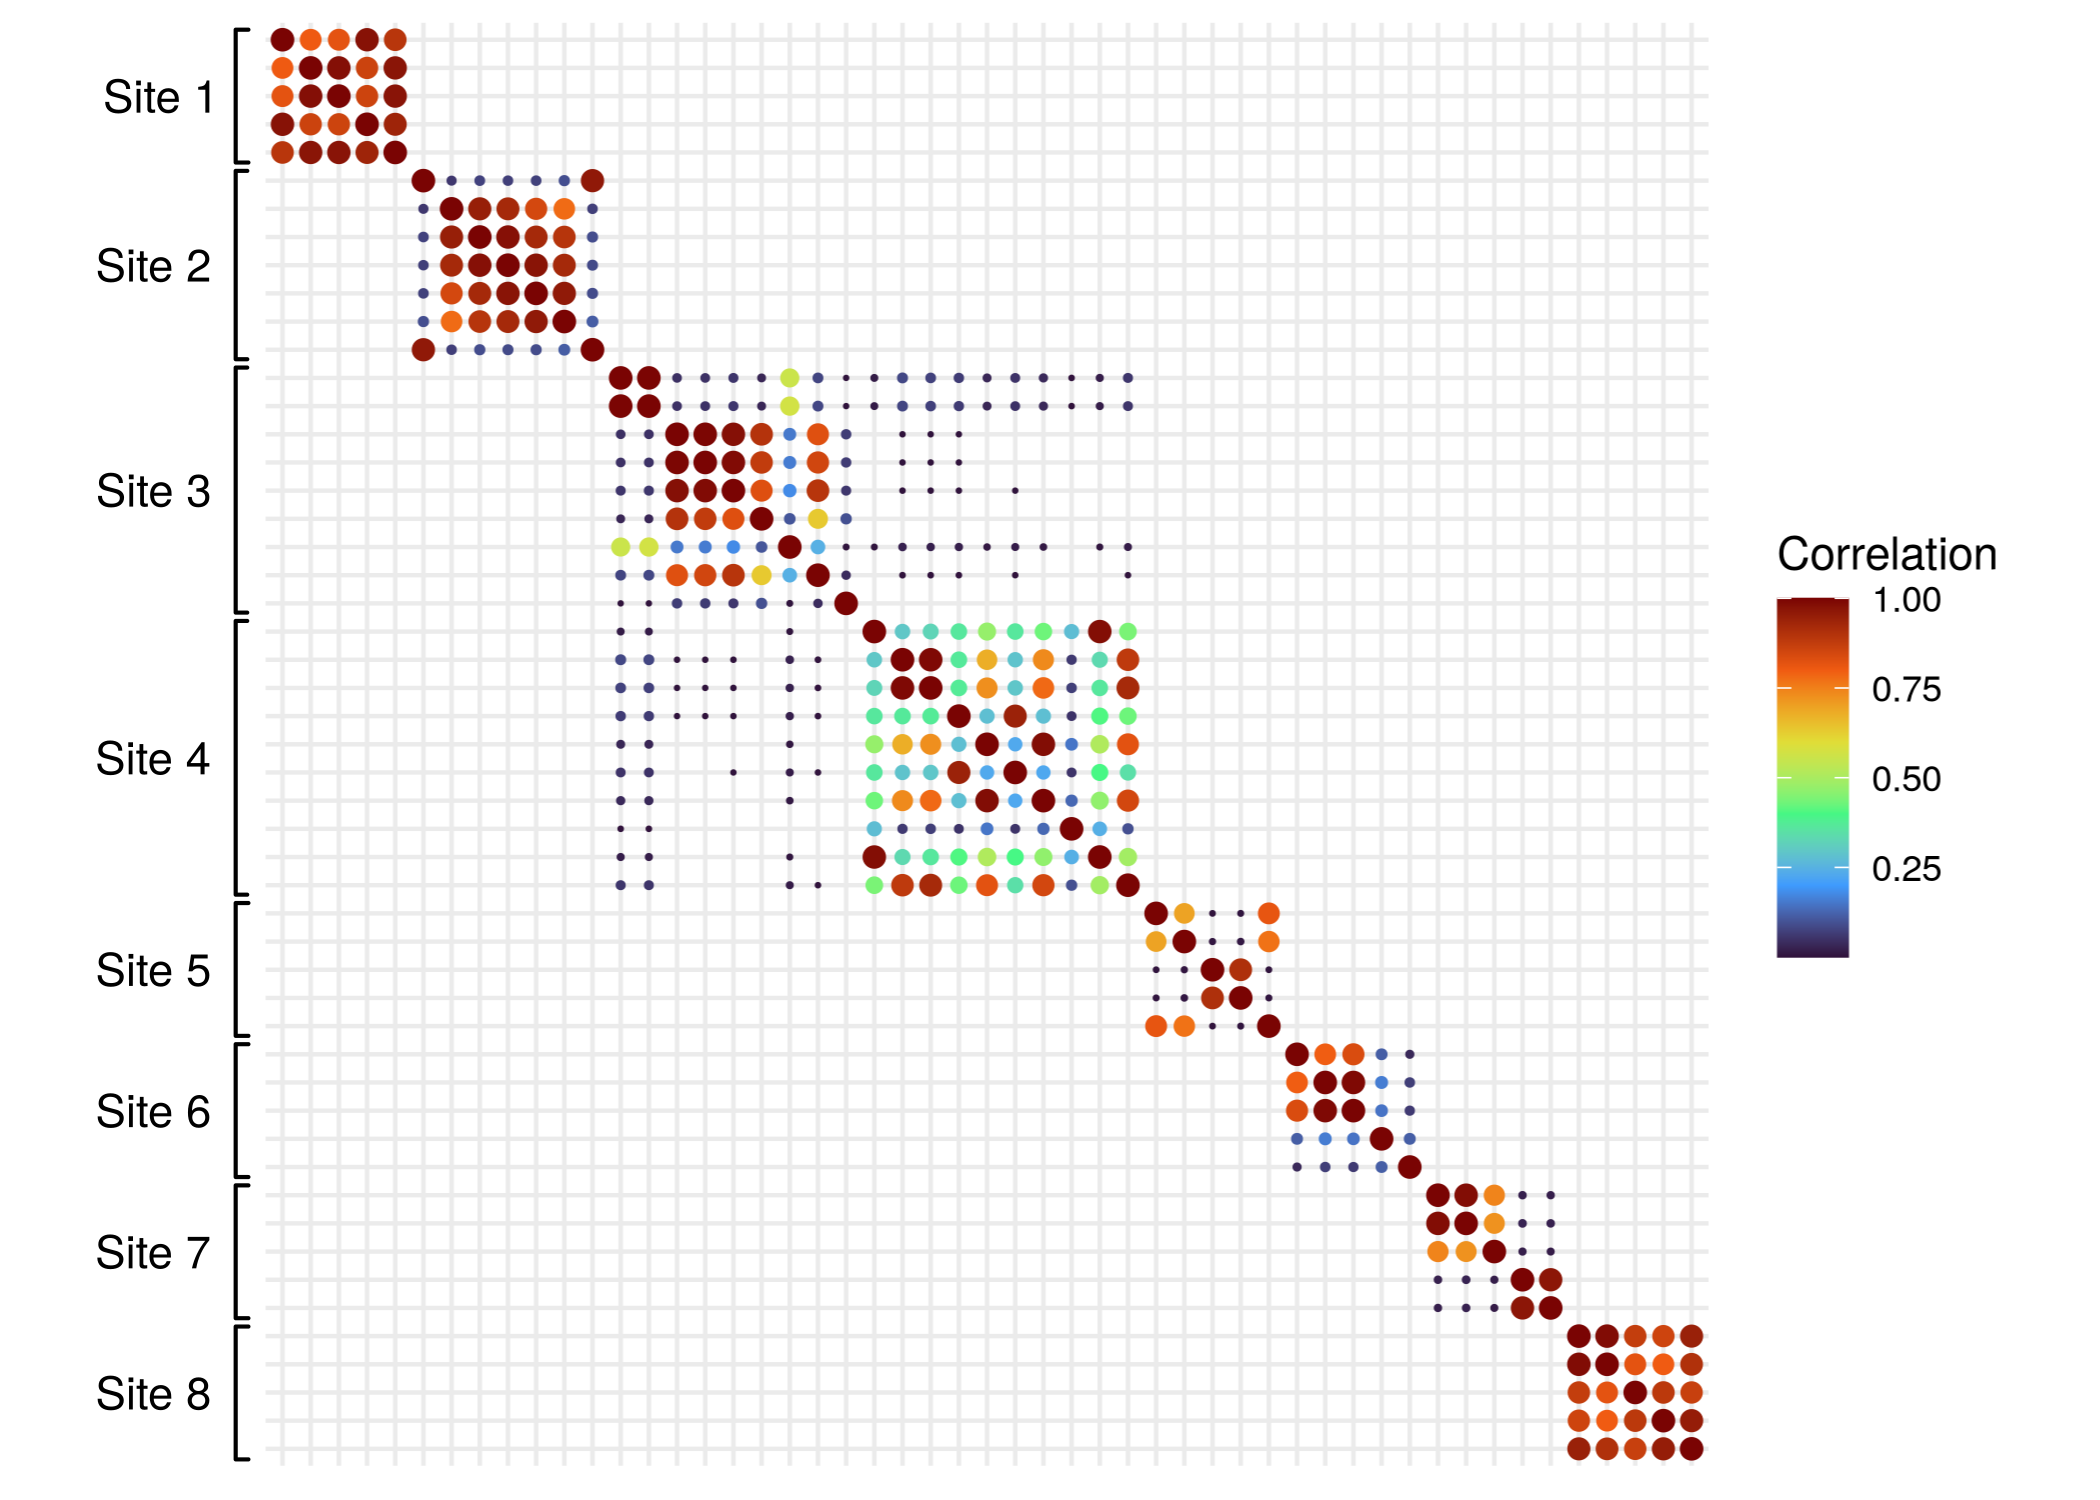
\includegraphics[width=.7\linewidth]{figures/rtg-correlation}
\caption{The assumed prior correlation matrix of the experimental plots of the RTG based on their geographical distance. The eight field sites of the RTG are located in Lower Saxony in northwest Germany. Originally, each site consisted of five experimental plots, but some of the plots had to be replaced due to storm and bark beetle damage. The correlation matrix is computed from the Matérn correlation function with range $\rho \approx 0.008$ (so that the correlation effectively decays to zero after 5 km) and smoothness $\nu = 1.5$. It is used with the latent Gaussian process representing the spatial effect in the structured additive predictor of the RTG multi-species count model.}
\label{fig:rtg-correlation}
\end{figure}

The non-parametric covariate effect is a spatial effect modeled as a Gaussian process, assuming a correlation structure between the experimental plots based on their geographical distance. The spatial effect accounts for unmeasured environmental and biological factors, hence capturing the otherwise unexplained variability in the data. The correlation matrix of the GP is computed from the Matérn correlation function with range $\rho \approx 0.008$ (so that the correlation effectively decays to zero after 5 km) and smoothness $\nu = 1.5$. Figure~\ref{fig:rtg-correlation} shows how the correlation matrix reflects the study design of the RTG with its eight field sites and five experimental plots per site. Most plots that are part of the same site are strongly correlated, while the correlation between the sites is effectively zero in most cases. In total, there are more than 40 plots, because some of the original plots had to be replaced due to storm and bark beetle damage.

Gaussian processes are stochastic processes, i.e.~collections of random variables, where every finite subset of the random variables has a joint multivariate normal distribution. They are popular both in machine learning and spatial statistics \citep{rasmussenGaussian2005}. In the context of spatial statistics, they are often used for kriging, a method for interpolating continuously indexed spatial data \citep{cressieStatistics1993}. Using a GP with the Matérn correlation function, a fixed range $\rho$ and the smoothness parameter $\nu = 1.5$, as we do in this application, is common practice when working with kriging and geoadditive models \citep{kammannGeoadditive2003}. One benefit of this approach is that only the variance (or smoothing) parameter $\tau^2$ needs to be estimated. Generally, the Matérn correlation function is considered to provide a good balance between smoothness and flexibility of the estimated processes.

\begin{table}
\centering
\caption{The widely applicable information criterion of the RTG multi-species count model for different taxa and count distributions. Note that the WAIC is reported on the log-score scale rather than the deviance scale, i.e.~higher values indicate a better predictive accuracy. For all taxa, the data shows some degree of overdispersion, making the location-scale parameterization of the negative binomial distribution a better fit than the Poisson distribution. The heavy-tailed Yule distribution performs better than the Poisson but worse than the negative binomial distribution for all studied taxa.}
\label{tab:rtg-waic}
\begin{tabular}{lrrrr}
\toprule
              & Count distribution &                 WAIC & Std. err. & Eff. param. \\
\midrule
Collembola    &  Negative binomial &  $\mathbf{-3281.88}$ &  $351.51$ &    $132.68$ \\
              &            Poisson &           $-3566.92$ &  $396.68$ &    $166.45$ \\
              &               Yule &           $-3384.62$ &  $356.98$ &    $129.74$ \\
\midrule
Small mammals &  Negative binomial &  $\mathbf{-2966.08}$ &  $237.28$ &     $31.11$ \\
              &            Poisson &           $-3330.91$ &  $281.24$ &     $61.55$ \\
              &               Yule &           $-3102.36$ &  $239.58$ &     $29.90$ \\
\midrule
Vegetation    &  Negative binomial & $\mathbf{-19022.28}$ & $3378.80$ &   $1028.34$ \\
              &            Poisson &          $-21016.58$ & $3627.85$ &   $1156.56$ \\
              &               Yule &          $-19174.55$ & $3390.47$ &   $1049.61$ \\
\bottomrule
\end{tabular}
\end{table}

For each taxon, we estimate the MSCM with the aforementioned structured additive predictor using three different count distributions for the total number of observations per experimental plot: the Poisson distribution, the negative binomial distribution in a location-scale parameterization \citep[Chapter~22.2.3]{rigbyDistributions2019}, and the Yule distribution \citep[Chapter~22.1.4]{rigbyDistributions2019}. The negative binomial distribution can account for potential overdispersion of the data compared to the standard Poisson distribution, while the Yule distribution is heavy-tailed. Comparing the different models by the WAIC, the negative binomial distribution shows the best performance across all taxa (Table~\ref{tab:rtg-waic}). For the vegetation data, the predictive accuracy of the heavy-tailed Yule distribution is almost as high as that of the negative binomial distribution, while the Poisson distribution seems to fit worst in all cases. For this reason, the presentation of the estimation results in the remainder of this section is only based on the MSCM with the negative binomial distribution.

\subsection{Estimation results}
\label{sec:results}

For each taxon and count distribution, the model was configured using Liesel and estimated using Goose, following the sampling scheme proposed in Section~\ref{sec:inference}. Four chains were sampled in parallel with 1000 warmup and 1000 posterior iterations. While sampling, the species richness and Shannon index on the plot and landscape-level were tracked to assess their posterior distribution. No thinning was applied to the chains before computing the summary statistics of the posterior distribution. For the collembola and vegetation data, the model was estimated without any errors and with a good effective sample size (ESS), while for the small mammal data, some divergent transitions of the NUTS kernels were observed. This is a consequence of the small mammal data being substantially smaller than the others with only seven species in total, four of which are very rare.

\begin{figure}
\centering
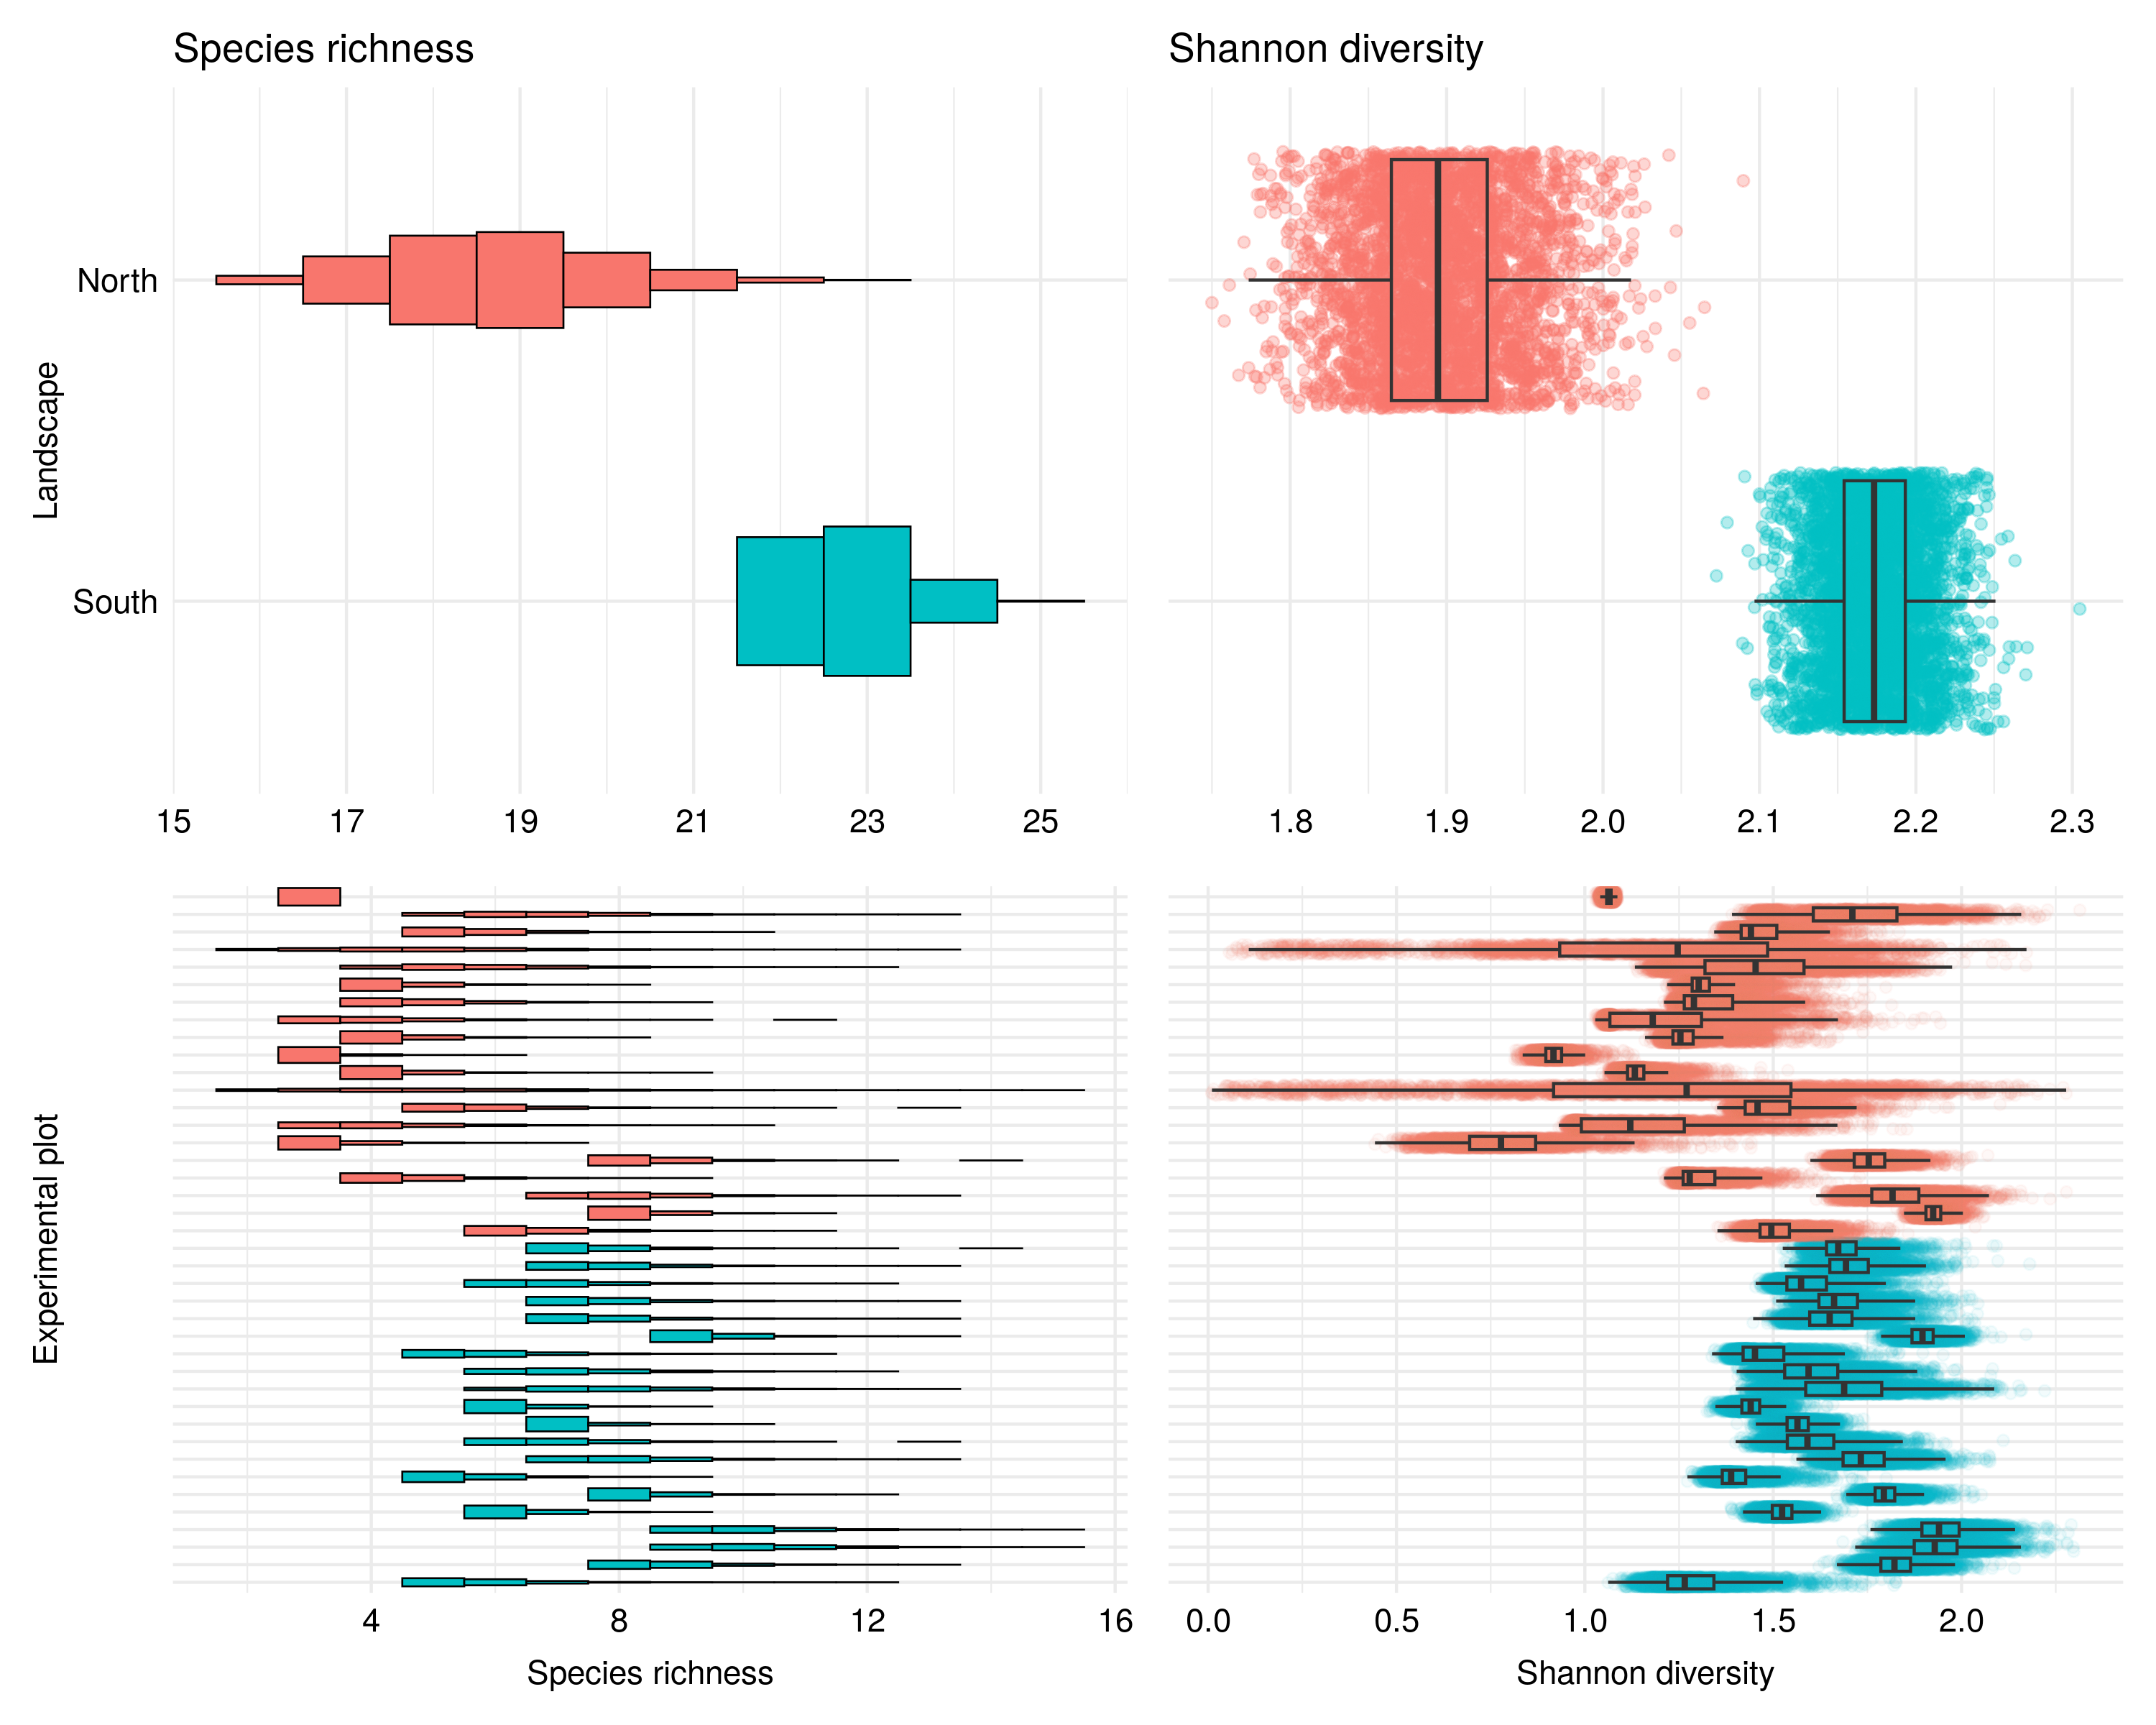
\includegraphics[width=\linewidth]{figures/rtg-diversity-col-geo}
\caption{The posterior distribution of the $\alpha$ and $\gamma$-diversity (on the plot and landscape-level) of collembola depending on the geographic location. The generally more favorable environmental conditions on the experimental plots in southern Lower Saxony are clearly reflected in a higher average species richness and Shannon index of collembola.}
\label{fig:rtg-diversity-col-geo}
\end{figure}

Our findings regarding the spatial effect on the species diversity are in line with \citet{glatthornSpecies2023}. For all three taxa, species richness and Shannon index are consistently estimated to be higher in southern Lower Saxony than in the north. Figure~\ref{fig:rtg-diversity-col-geo} shows the posterior distribution of both diversity indices on the plot and landscape-level for collembola. The differences between the northern and southern plots are generally very pronounced for collembola and for the vegetation. For small mammals, the posterior distribution also indicates a slightly higher species diversity in the south, but as the number of observed small mammal species is generally very low (posterior mean of 7.0 of the landscape species richness in the south, 5.32 in the north), the difference is quite hard to identify.

\begin{figure}
\centering
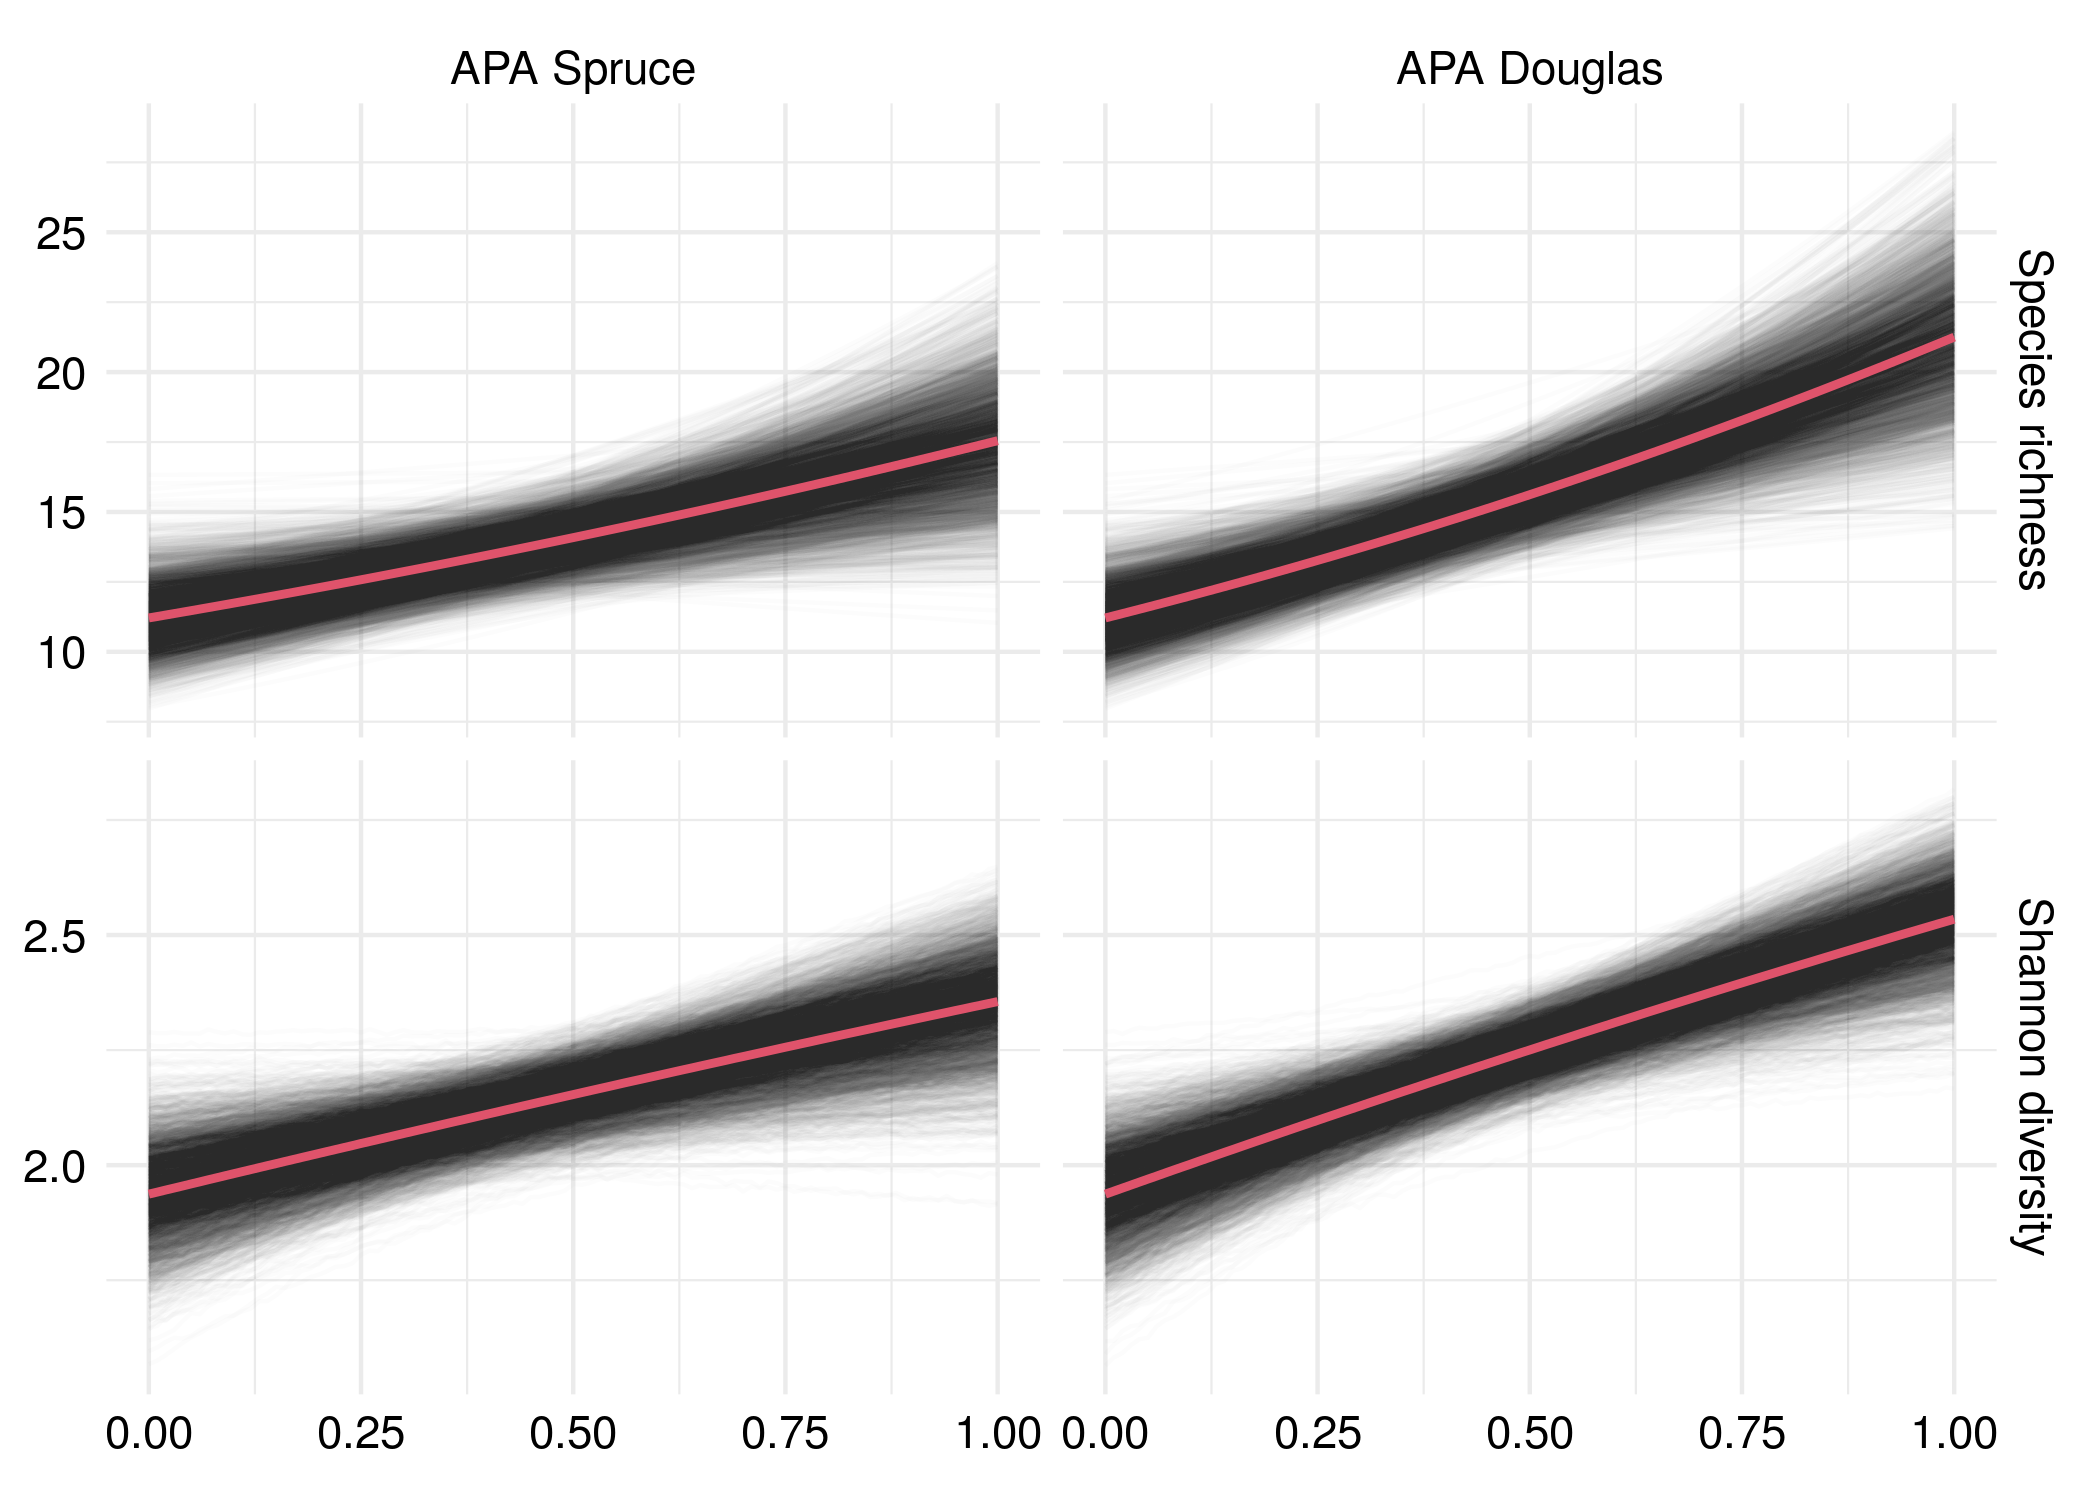
\includegraphics[width=.7\linewidth]{figures/rtg-diversity-veg-apa}
\caption{The posterior distribution of the effect of the composition of tree species on the $\alpha$-diversity (on the plot-level) of the overall vegetation on the experimental plots. The composition of tree species is measured in terms of the area potentially available (APA, computed from a weighted Voronoi tessellation of the plot) for the different species. A higher APA for the coniferous species Norway spruce and Douglas fir corresponds with a higher average species richness and Shannon index of the vegetation on the plots. This effect is even more pronounced for Douglas fir than for Norway spruce.}
\label{fig:rtg-diversity-veg-apa}
\end{figure}

The impact of the combination of tree species on the species diversity remains somewhat ambiguous. The diversity of collembola shows a trend towards a reduced species richness and Shannon index with a higher APA for spruce and Douglas fir. However, the posterior variance of the effect is high, indicating a substantial estimation uncertainty. In contrast, the diversity of small mammals and the vegetation appears to increase with a higher APA for the coniferous species. While for small mammals, the estimation uncertainty remains high, the positive effect on the vegetation is rather pronounced, as shown in Figure~\ref{fig:rtg-diversity-veg-apa}. \citet{glatthornSpecies2023} report a similar pattern across the taxa collembola, small mammals and vegetation.

The model specification presented in this section only allows for the estimation of the species effect of spruce and Douglas fir relative to beech. The effect of mixed stands compared to pure stands cannot be assessed with this parameterization. To address this question, a non-linear effect of the APA of spruce and Douglas fir on the structured additive predictor for the occupancy probabilities would need to be assumed and modeled using e.g.~polynomials or P-splines. The figures illustrating the spatial effect and the effect of the composition of tree species on the diversity of the taxa omitted in the article may be found in the supplementary material.

\section{Conclusion}
\label{sec:conclusion}

In conclusion, this study introduces the multi-species count model as a new model class for assessing the relationship between site conditions and species diversity. The model allows us to incorporate a structured additive predictor with linear, non-linear, random and spatial effects describing the site conditions. It can be estimated with a fully Bayesian inference scheme based on an efficient MCMC algorithm, which we evaluate in a simulation study with different scenarios and apply to data from a large-scale ecological research project in Lower Saxony, Germany.

We use the model to study the effect of admixing two coniferous species on the ecosystem in European beech forests, accounting for the spatial correlation between the field sites. This application demonstrates the usefulness of the model in real-world scenarios, where it can provide insights into the complex relationships between species diversity and site conditions. Generally, the model can be applied to a broad range of problems, including the analysis of different species diversity indices and taxa. It can be used to estimate both the occupancy probabilities and the expected abundances of the studied species. Due to its low data requirements, it is a particularly useful tool for meta-studies across various taxa that are sampled according to different study designs.

Modeling species compositions and their driving environmental factors via species occupancy probabilities, and aggregating them in ecologically meaningful indices in a Bayesian framework offers unique flexibility in terms of research questions that can be addressed in a consistent way. For example, analyses of contrasts between different species groups (rare vs.~common, specialists vs.~generalists, etc.) or of trait compositions of species communities depending on environmental factors can all be derived from the same model. Through sampling from the posterior predictive distribution conditional on environmental factors, simulation studies about the impact of different landscapes on the overall species composition can be carried out easily.

Several aspects deserve further attention in future research: One key aspect to consider is the extension of the model specification with another structured additive predictor for the expected abundances of the species, potentially introducing a functional relationship between the new and the old predictor for the occupancy probabilities. Moreover, alternative parameterizations and count distributions for the total number of observations per experimental plot could be explored. It should be noted that, unlike multi-species occupancy models, our model lacks the ability to disentangle the detection probabilities and expected abundances of the species. The current version of the model also cannot estimate the size of a meta-community accounting for unobserved species. To overcome these limitations, more complex versions of the model could be developed in the future.

Overall, the proposed multi-species count model provides a flexible and powerful framework for the analysis of species diversity data, and can be used to identify key environmental drivers of biodiversity patterns. Our study contributes to the growing body of literature highlighting the potential of Bayesian hierarchical modeling in ecology. The multi-species count model can be applied to many different datasets, and we hope it will stimulate further research in the field of community ecology.

\clearpage
\nocite{tangeGNU2023}
\bibliographystyle{plainnat}
\bibliography{references}

\clearpage
\section*{Supplementary material}

In this supplementary material, we present additional figures that are not included in the article ``A Structured Additive Multi-Species Count Model for Assessing the Relation Between Site Conditions and Species Diversity''. The figures show the estimation results for the taxa that are omitted from Section~\ref{sec:application}, i.e.~the application on species diversity in mixed forest stands in Lower Saxony, Germany. Specifically, the spatial effect, i.e.~the posterior distribution of species diversity depending on the geographic location, and the tree species effect, i.e.~the posterior distribution of the effect of the composition of tree species on species diversity, are shown. See Section~\ref{sec:results} for more details on the interpretation of the figures.

\subsection*{Spatial effect}

\begin{figure}[ht!]
\centering
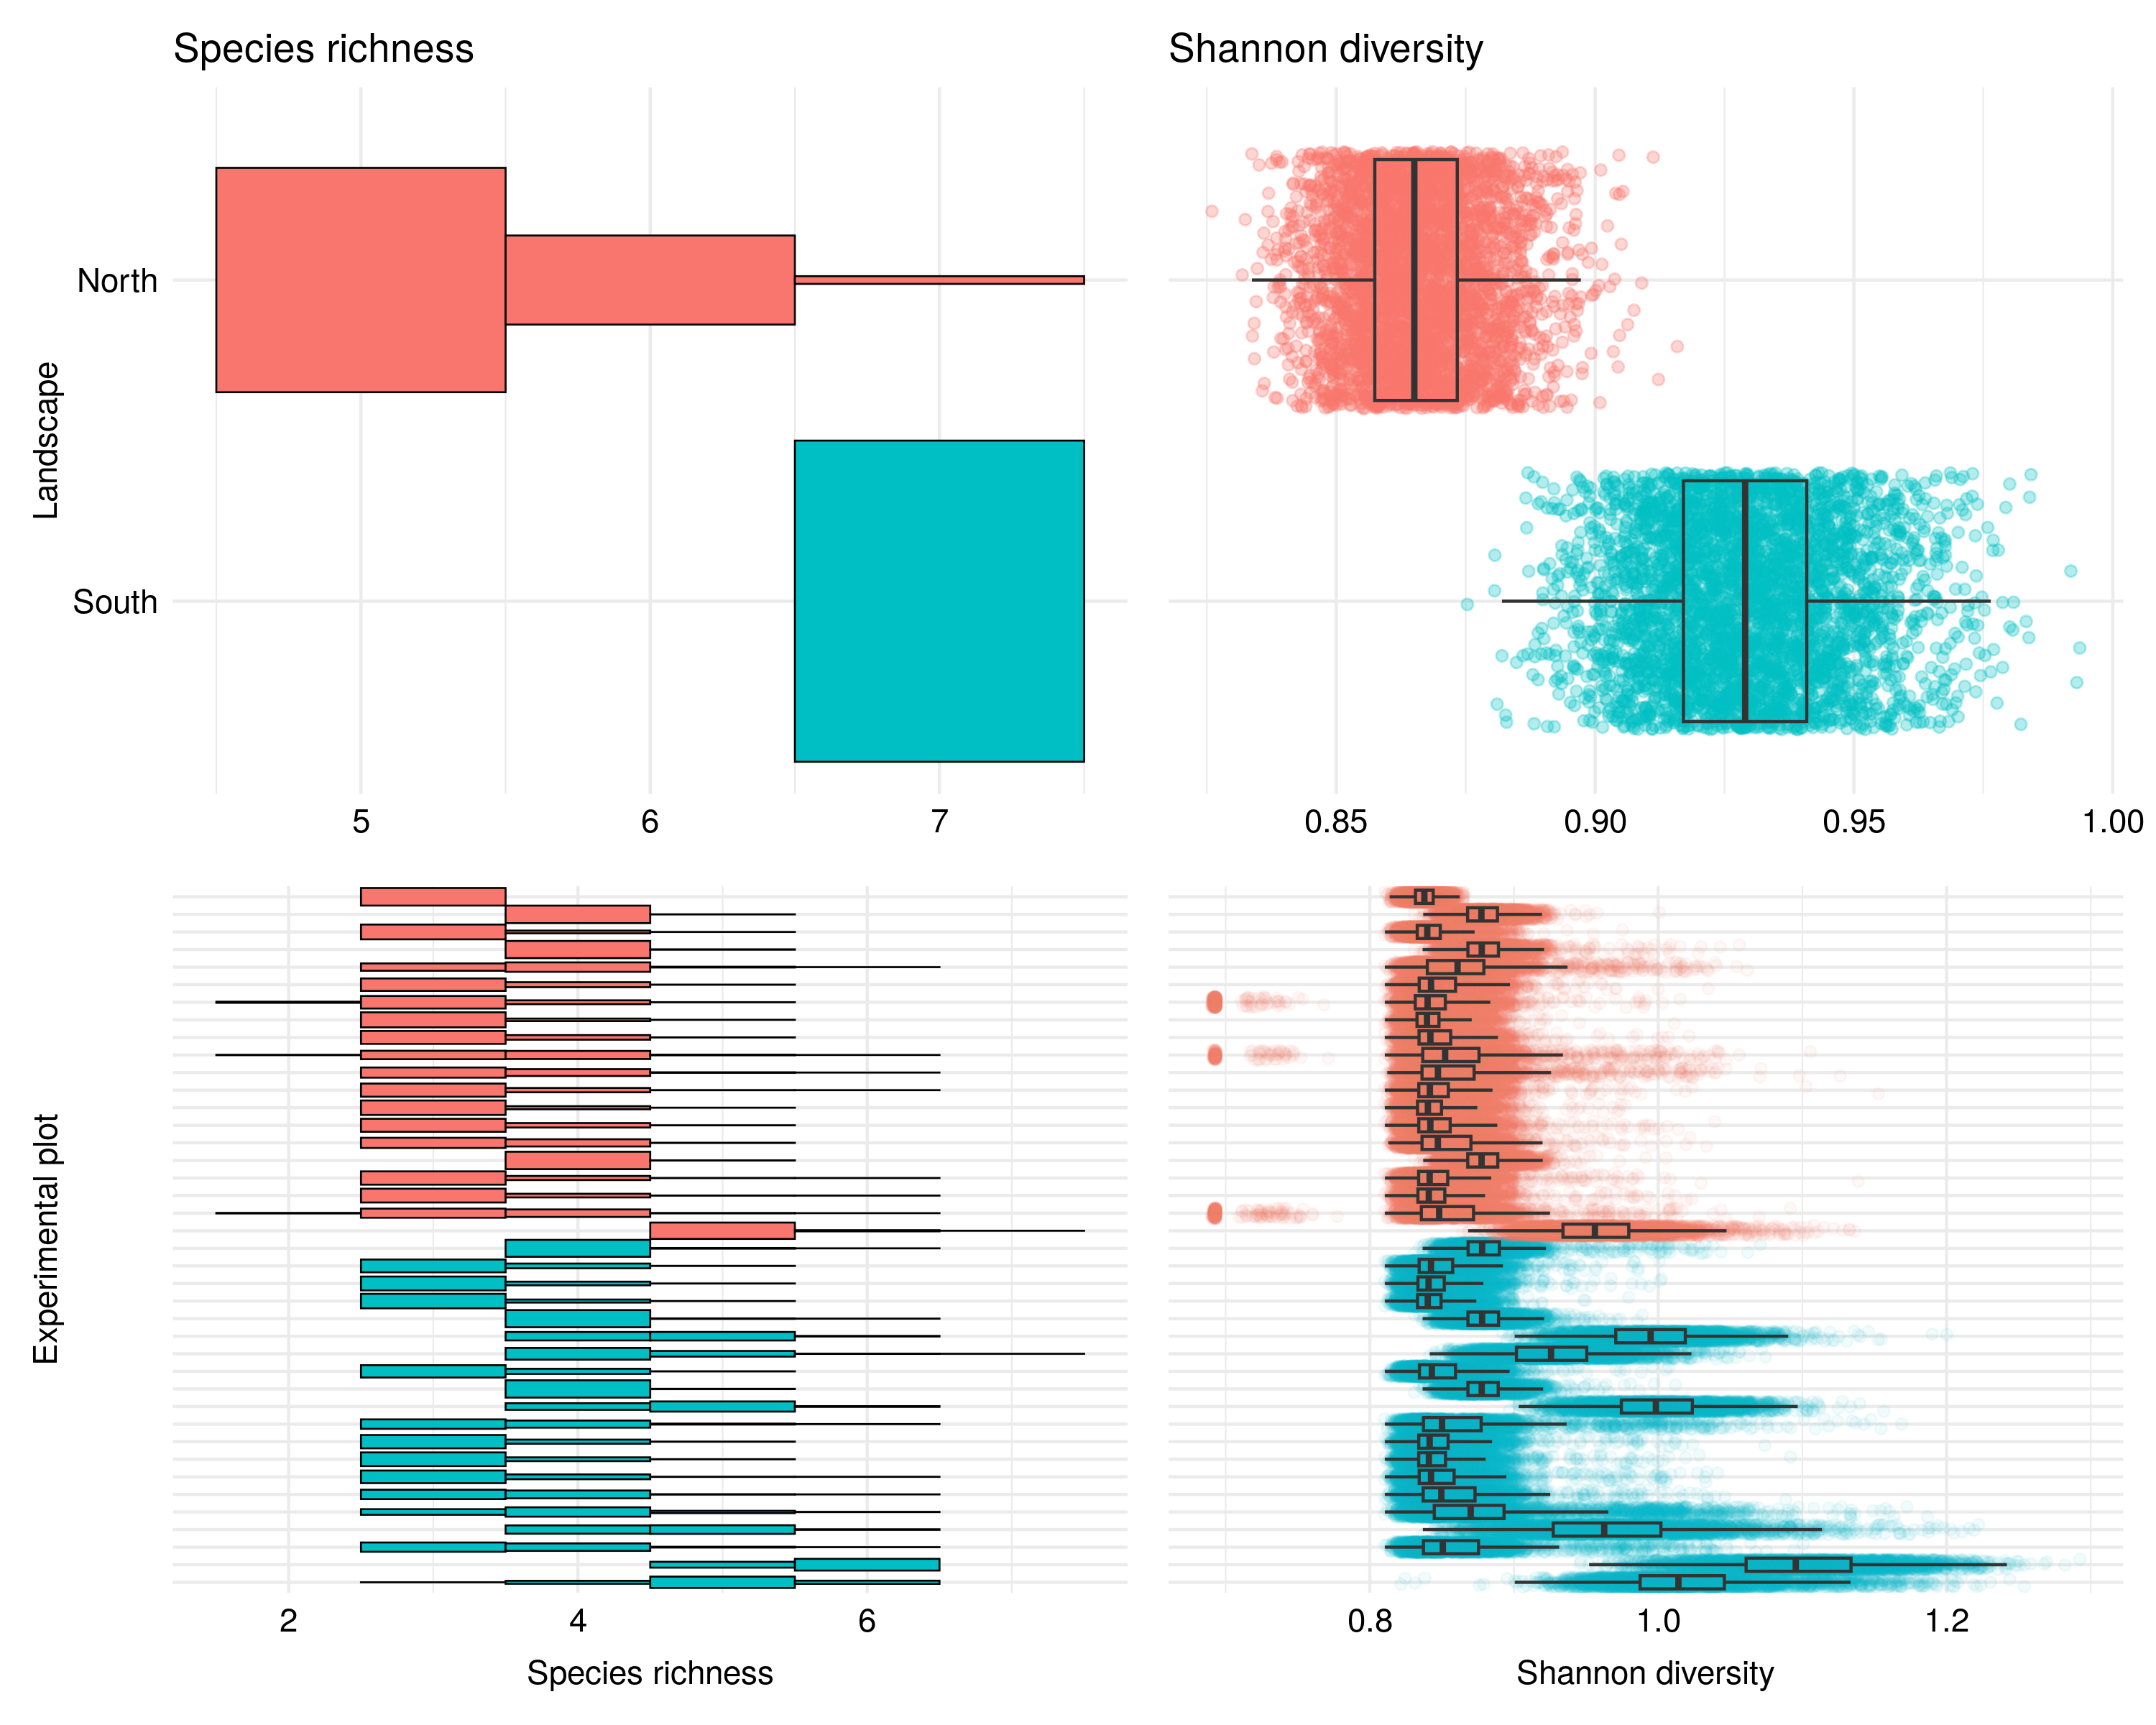
\includegraphics[width=\linewidth]{figures/rtg-diversity-sma-geo}
\caption{The posterior distribution of the $\alpha$ and $\gamma$-diversity (on the plot and landscape-level) of \textbf{small mammals} depending on the geographic location.}
\label{fig:rtg-diversity-sma-geo}
\end{figure}

\begin{figure}[ht!]
\centering
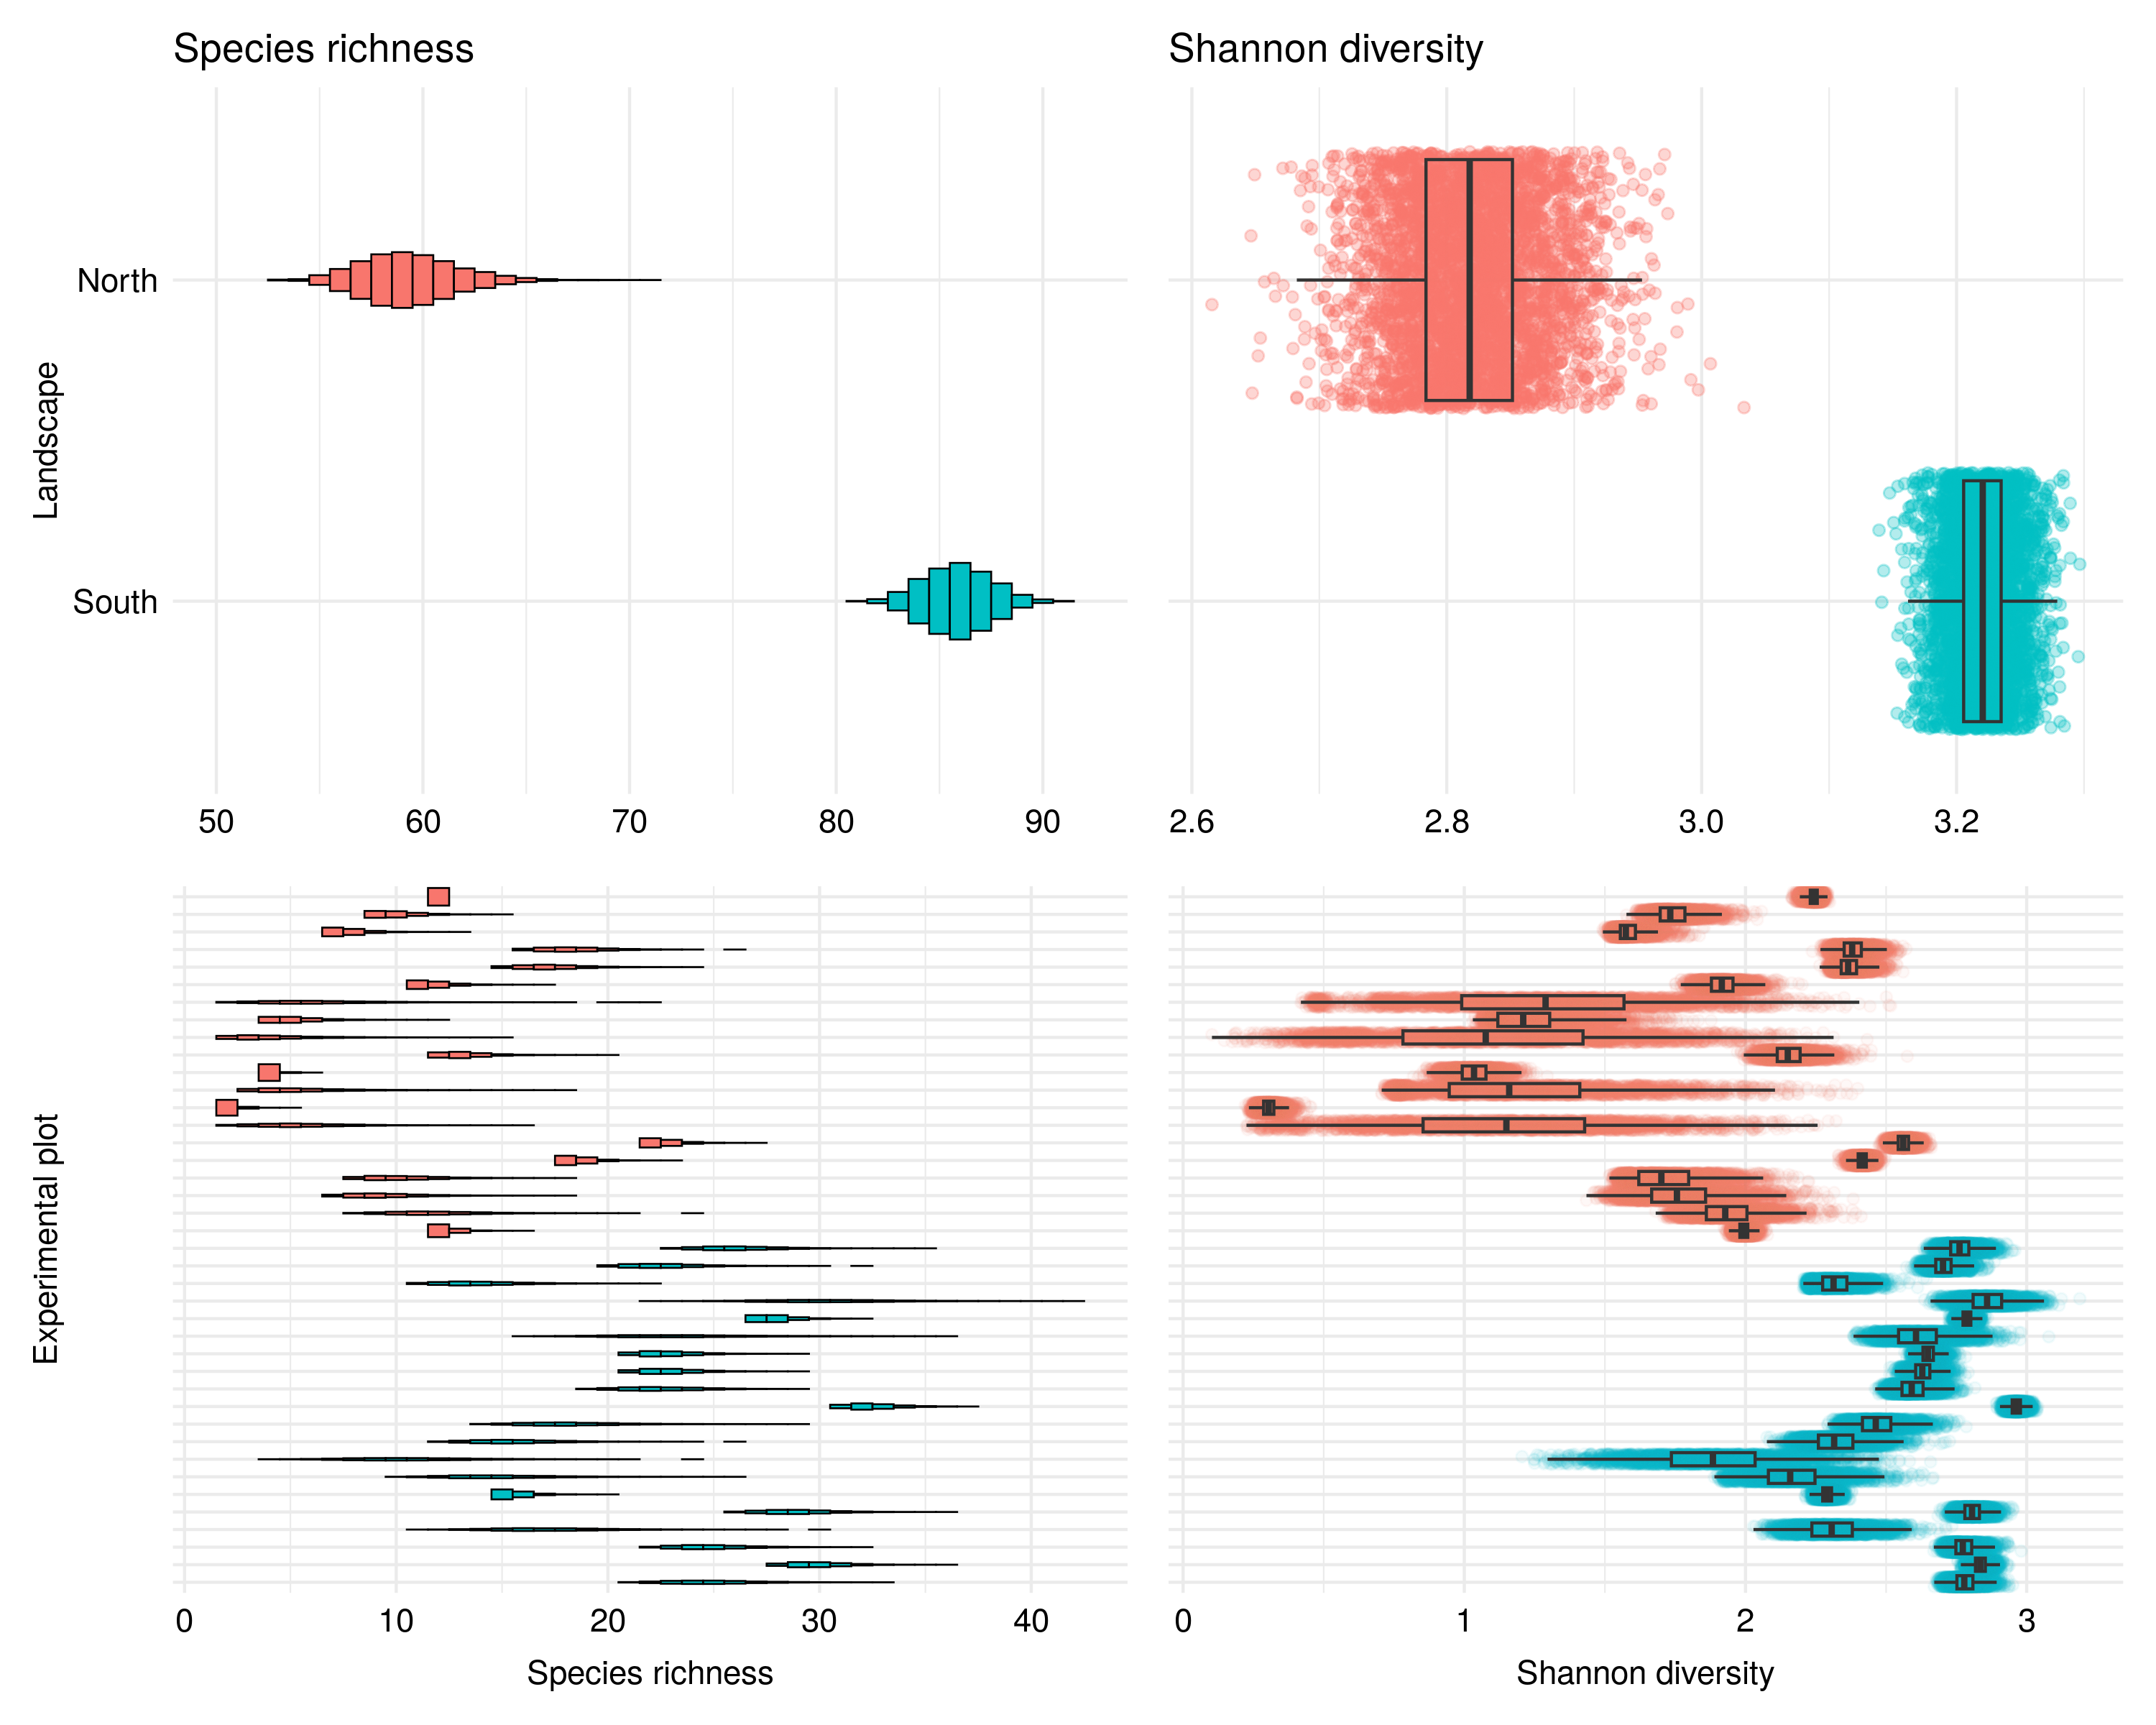
\includegraphics[width=\linewidth]{figures/rtg-diversity-veg-geo}
\caption{The posterior distribution of the $\alpha$ and $\gamma$-diversity (on the plot and landscape-level) of the \textbf{vegetation} depending on the geographic location.}
\label{fig:rtg-diversity-veg-geo}
\end{figure}

\clearpage
\subsection*{Tree species effect}

\begin{figure}[ht!]
\centering
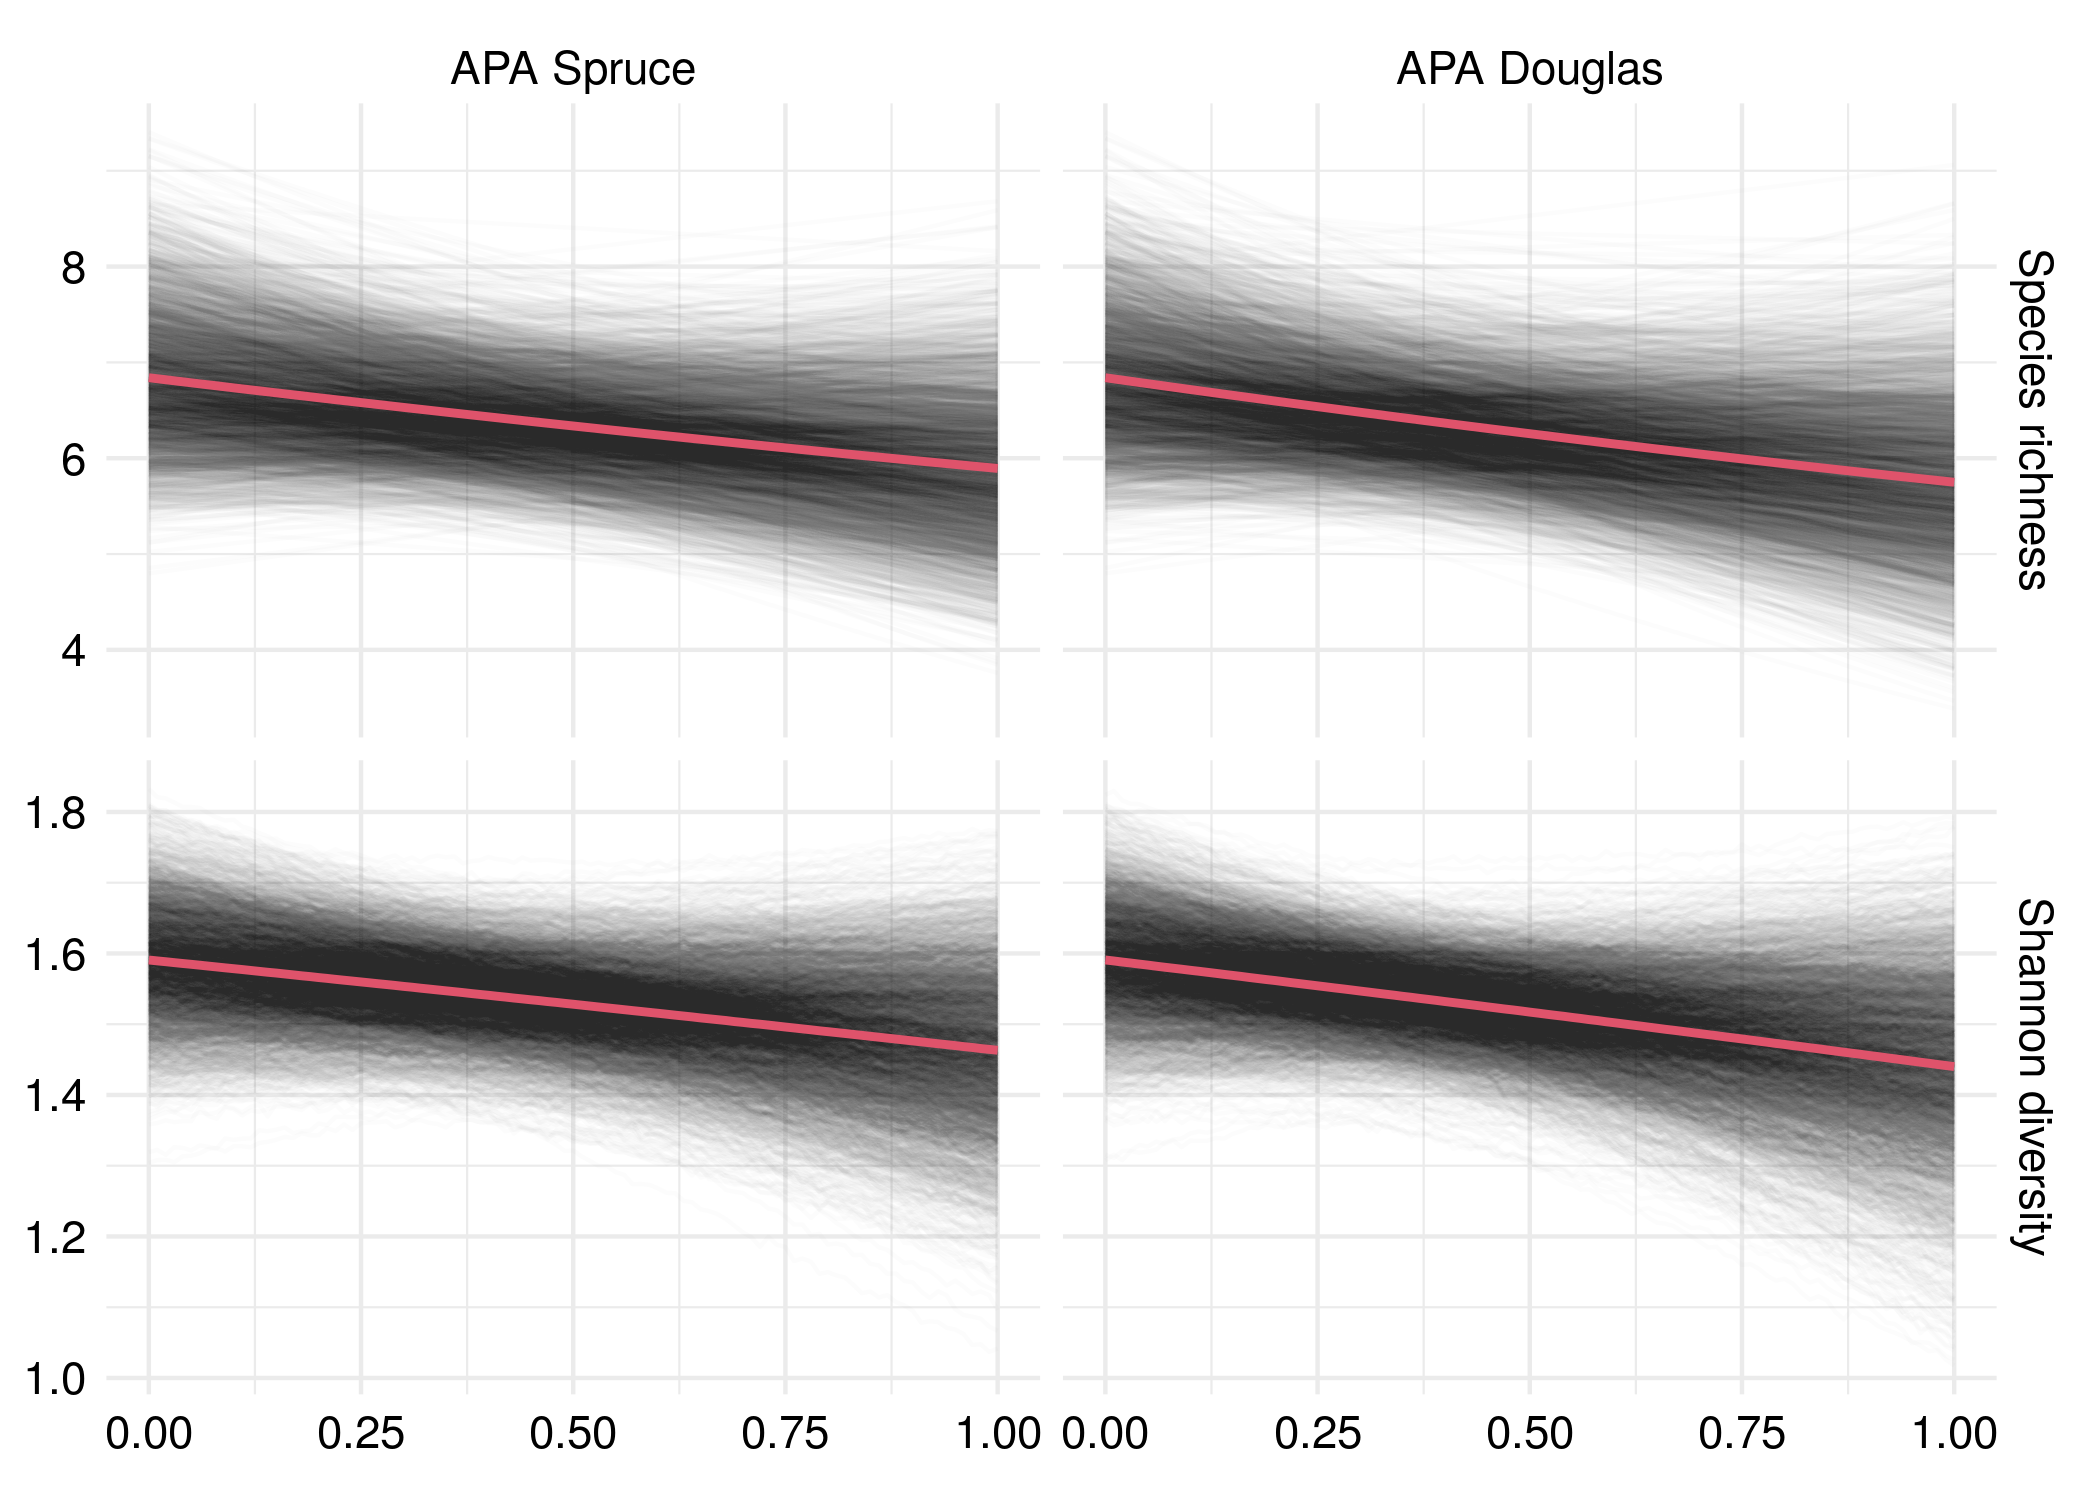
\includegraphics[width=.7\linewidth]{figures/rtg-diversity-col-apa}
\caption{The posterior distribution of the effect of the composition of tree species on the $\alpha$-diversity (on the plot-level) of \textbf{collembola} on the experimental plots.}
\label{fig:rtg-diversity-col-apa}
\end{figure}

\begin{figure}[ht!]
\centering
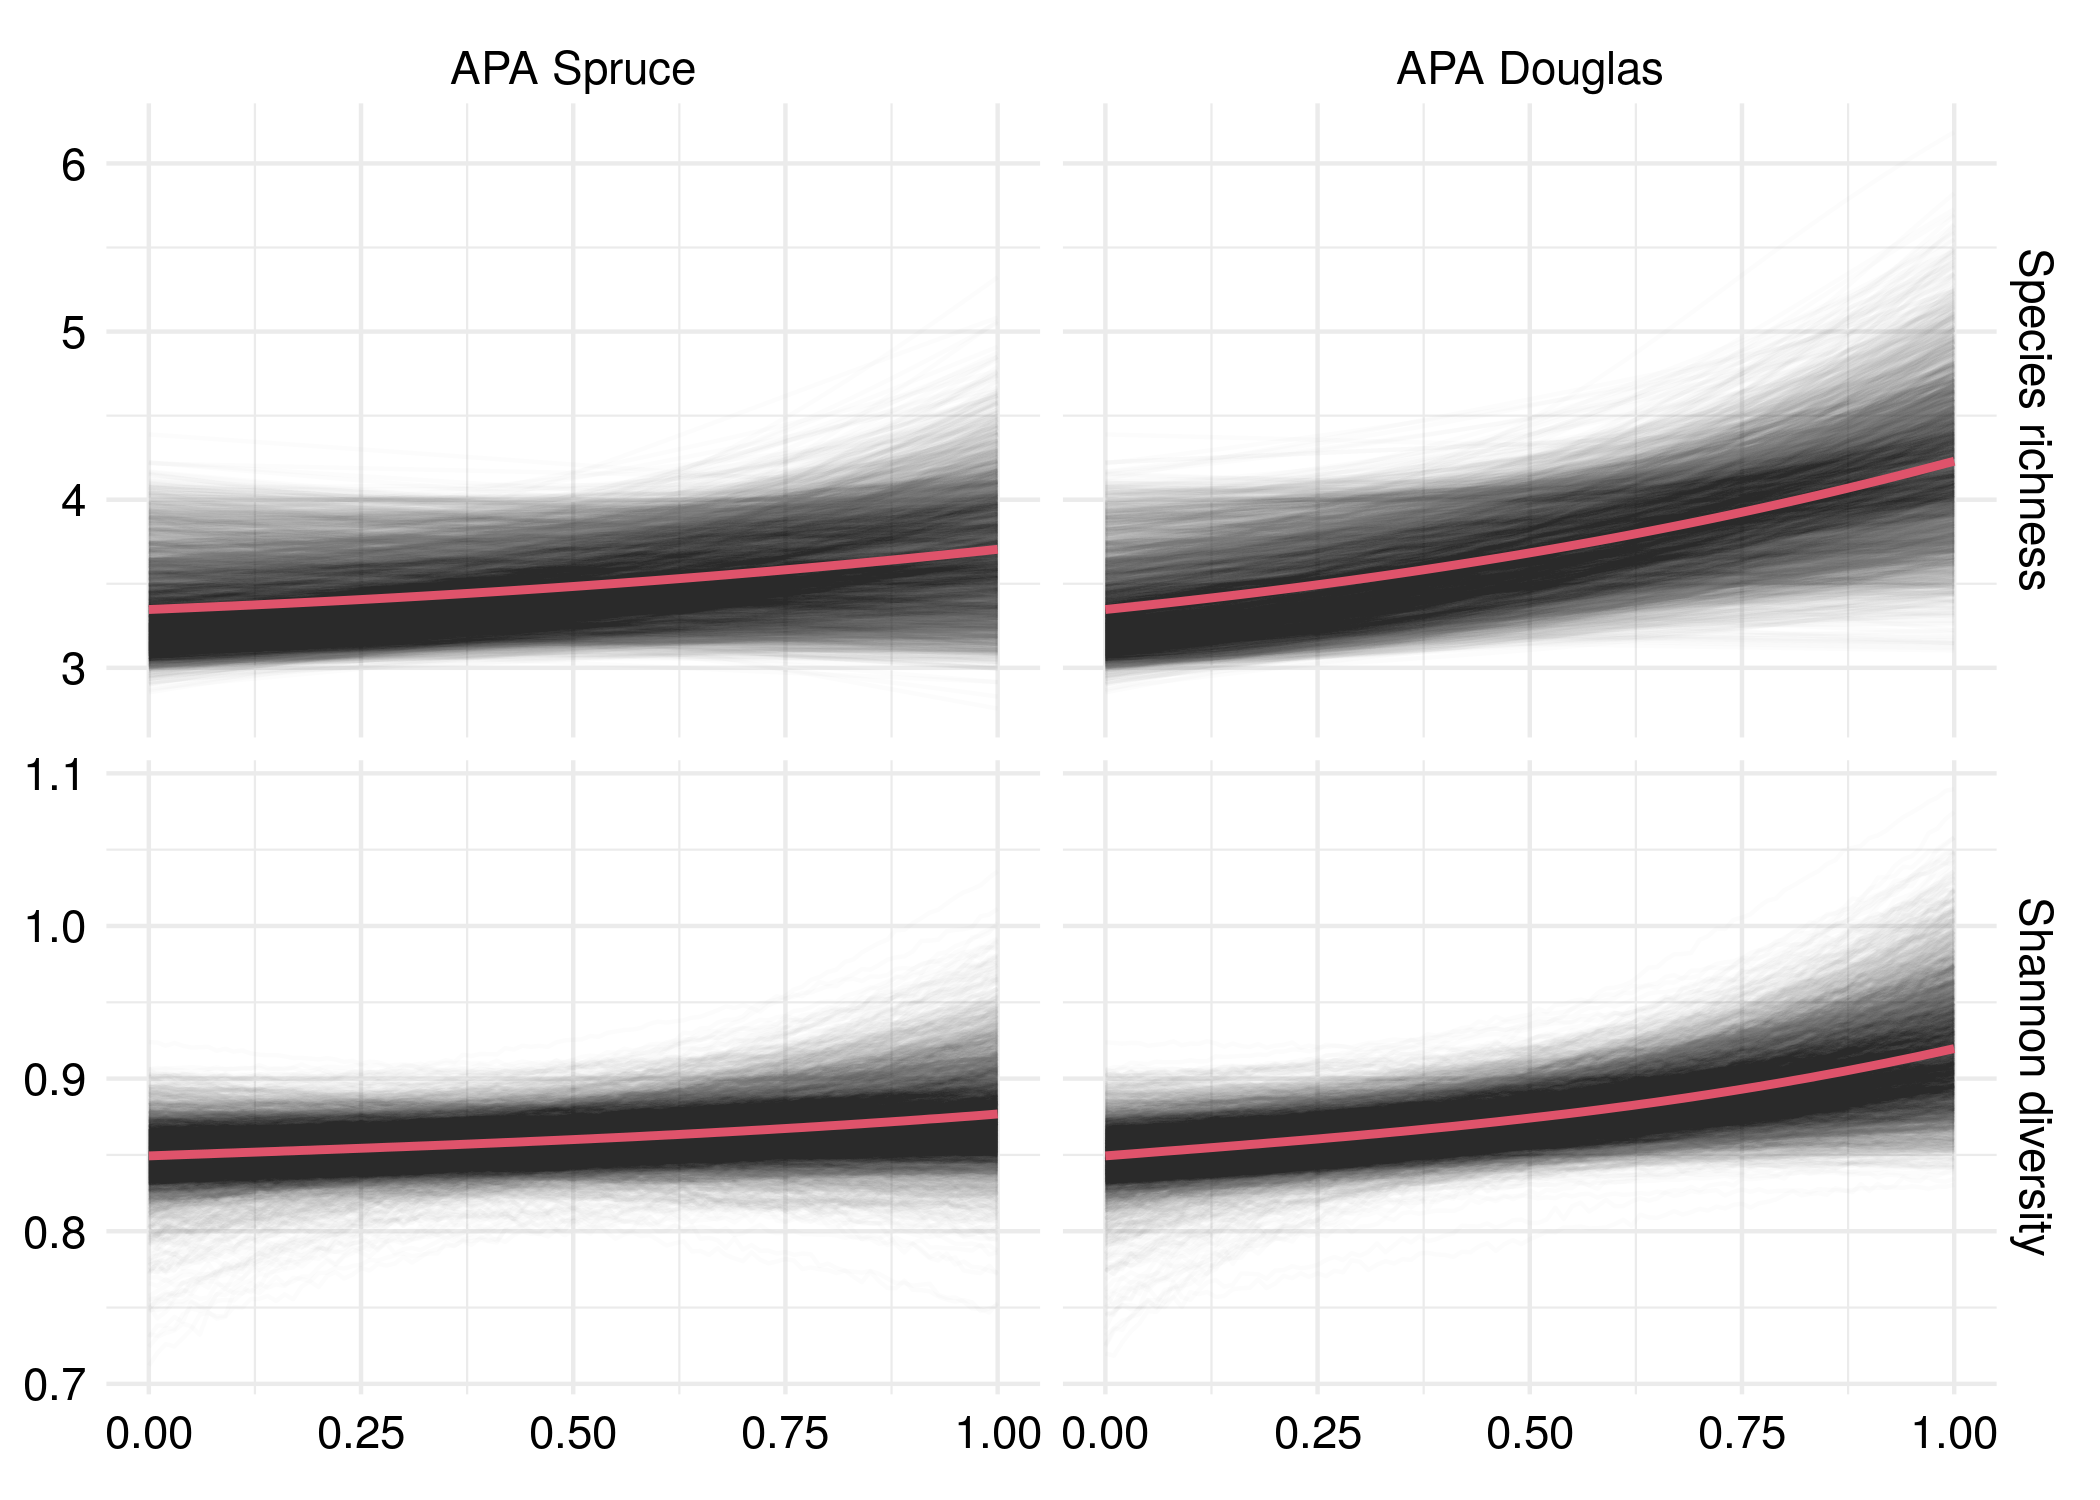
\includegraphics[width=.7\linewidth]{figures/rtg-diversity-sma-apa}
\caption{The posterior distribution of the effect of the composition of tree species on the $\alpha$-diversity (on the plot-level) of \textbf{small mammals} on the experimental plots.}
\label{fig:rtg-diversity-sma-apa}
\end{figure}

\end{document}
